%------chapter 2: literature review
\chapter{روش‌های پیشین} \label{chap:lr}
در این فصل ابتدا یک چارچوب کلی برای روش‌های مورد استفاده در یادگیری بدون برد توصیف می‌شود. سپس روش‌های موجود طبق این چارچوب دسته‌بندی شده و مرور خواهند شد.


از نظر تاریخی، پیش از تعریف و بیان رسمی مسئثه یادیگری بدون برد، استفاده از اشتراک و تمایز برخی ویژگی‌ها میان دسته‌های مختلف در بینایی ماشین مورد بررسی قرار گرفته است
\cite{BakkerH03, TsochantaridisJHA05, ulman2005}،
اما این روش‌ها به شناسایی دسته‌های کاملا جدید از روی این ویژگی‌ها توجه نشان نداده‌اند.
مسئله‌ی یادگیری تک‌ضرب\LTRfootnote{One-shot Learning}
هم یک مسئله نزدیک به یادگیری بدون برد است که پیش‌تر مورد بررسی بوده است
\cite{miller12}.
در حقیقت می‌توان یادگیری تک‌ضرب را حالت خاصی از یادگیری بدون برد در نظر گرفت که در آن توصیف دسته‌های دیده نشده به صورت یک نمونه از آن دسته ارائه شده است
\cite{bengio08}.
 پدیده شروع سرد\LTRfootnote{cold start}
 در سامانه‌های توصیه‌گر\LTRfootnote{Recommender Systems}
 را نیز می‌توان از حالت‌های خاص یادگیری بدون برد در نظر گرفت که در آن برای یک کاربر یا مورد جدید پیشنهاد صورت می‌گیرد.


بیان مسئله  یادگیری بدون برد به طور رسمی برای اولین بار در
\cite{bengio08}
صورت گرفت. در آن‌جا دو رویکرد کلی برای حل مسئله یادگیری بدون برد بیان می‌شود. یک روش که رویکرد فضای ورودی\LTRfootnote{input space view}
نامیده می‌شود، سعی در مدل کردن نگاشتی با دو ورودی دارد. یک ورودی نمونه‌ها و دیگری توصیف دسته‌ها و امتیازی مبنی بر مطابقت آن‌ها با یکدیگر تولید می‌کند، یعنی برای نمونه‌ها و توصیف‌های مربوط به یک دسته امتیاز بالا و برای نمونه‌ها و توصیفاتی که متعلق به دسته‌ی یکسانی نیستند مقادیر کوچکی تولید می‌کند. با تخمین زدن چنین نگاشتی روی داده‌های آموزش، دسته‌بندی نمونه‌های آزمون در دسته‌هایی که تا کنون نمونه‌ای نداشته‌اند ممکن خواهد شد. به این صورت که هر نمونه با توصیف دسته‌های مختلف به این تابع داده شده و متعلق به دسته‌ای که امتیاز بیشتری بگیرد، پیش‌بینی خواهد شد.
در روش دیگر که رویکرد فضای مدل\LTRfootnote{model space view}
نام دارد، مدل مربوط به هر دسته (برای مثال پارامترهای دسته‌بند مربوط به آن)، به عنوان تابعی از توصیف آن دسته در نظر گرفته می‌شود.

ما در این فصل از دسته‌بندی دیگری برای مرور روش‌های پیشین استفاده می‌کنیم. برای این کار ابتدا معرفی یک چارچوب کلی برای انجام یادگیری بدون برد لازم است که دو رویکرد فوق نیز در این چارچوب قابل بیان هستند.
 % چارچوبی که در ادامه می‌آید بر این اساس استوار است که تصاویر و توصیفات آن‌ها به یک فضای مشترک نگاشته می‌شوند. اگر بخواهیم دو دسته‌ی بالا در را در با این بیان توصیف کنیم، در رویکرد فضای ورودی، فضای مشترک فضایی است که نگاشت شباهت سنجی، ضرب داخلی آن فضاست و در رویکرد فضای مدل، فضای مشترک فضای دسته‌بندها خواهد بود.

 می‌توان گفت که هر روش برای یادگیری بدون برد از سه قسمت تشکیل شده است که ممکن است به صورت مستقل یا همزمان انجام شوند؛ این سه قسمت عبارتند از:
\begin{enumerate}
  \item یادگرفتن نگاشتی از فضای تصاویر به فضای مشترک
  که آن را با $\phi$ نشان می‌دهیم.
  \item نگاشت توصیف‌ها به فضای مشترک
  که آن را با $\theta$ نشان می‌دهیم.
  \item
   ارائه روشی برای تعیین مشابهت در این فضای مشترک و اختصاص برچسب به تصاویر.
\end{enumerate}

\section{نماد‌گذاری}\label{notaion}
برای این که توصیف دقیق روش‌های پیشین ممکن باشد، در ابتدای یک نمادگذاری برای مسئله ارائه می‌دهیم و از آن برای بیان مرور روش‌های پیشین و بیان روش پیشنهادی در فصل آینده استفاده خواهیم کرد.

برای ماتریس $X$،    
$X_{(i)}$
 سطر $i$م آن و 
$\normf{X}$
نرم فروبنیوس آن را نشان می‌دهد. هم‌چنین برای بردار $\mathbf{x}$،
 $x_i$ 
 درایه‌ی $i$م را نشان می‌دهد.
    ضرب داخلی با نماد  $\langle ., . \rangle $ نشان داده شده است.
$diag(\mathbf{x})$
یک ماتریس قطری  را نشان می‌دهد که بردار $\mathbf{x} $ روی قطر اصلی آن قرار داده شده است.  $\mathbf{1}$ یک بردار تمام یک و $\mathbf{1}_k$ یک بردار که عنصر $k$م آن یک و سایر عناصر آن صفر است را نشان می‌دهند. 

 تصاویر را با
 $\mathbf{x}  \in \mathbb{R}^d$
 نشان می‌دهیم که $d$ ابعاد داده را نشان می‌دهد. توصیف‌ها را با
 $ \mathbf{c}  \in \mathbb{R}^a$
 نمایش می‌دهیم که  $a$ ابعاد توصیف‌هاست. مجموعه دسته‌های دیده‌شده را با  $ \mathcal{S}$ و دسته‌های دیده‌نشده را با $ \mathcal{U}$ و مجموعه کل برچسب‌ها را با $ \mathcal{Y}$
 نشان می‌دهیم که
 $ \mathcal{Y} =  \mathcal{U} \cup \mathcal{S} $.
 تعداد دسته‌های آموزش را با $n_s$ و تعداد دسته‌های آزمون را با $n_u$ نشان می‌دهیم.
هم‌چنین   $\mathbf{c_y} $ که در آن    $ y \in \mathcal{U} \cup \mathcal{S} $ بردار توصیف دسته $y$ را نشان می‌دهد.

    فرض می‌کنیم در زمان آموزش 
    $ \{ (\mathbf{x_i, y_i}) \}_{i=1}^{N_s} $
     شامل $N_s$
     تصویر از دسته‌های دیده شده به همراه برچسب  موجود است.
     $X_s \in \mathbb{R}^{d \times N_s }$
  ماتریس مجموعه تصاویر و $Y_s$ ماتریس برچسب‌های داده‌های آموزش با نمایش یکی یک
  \LTRfootnote{One-Hot Encoding}
   است.  هم‌چنین توصیف‌های هر کدام از دسته‌های آموزش،
  $C_s \in \mathbb{R}^{s \times a}$
 نیز موجود است. $X_u$ و $C_u$ بطور مشابه برای دسته‌های آزمون تعریف می‌شوند.
$ X = [X_s;X_u]$
ماتریس ویژگی تمام نمونه‌ها، اعم از آموزش و آزمون است.


   


\section{کران خطا}\label{bound}
تعریف و فرضیات یادگیری از صفر با حالت معمول دسته‌بندی متفاوت است. در نتیجه کران‌هایی که پایین بودن خطای دسته‌بندی را با استفاده تعداد محدودی نمونه ضمانت می‌کنند در اینجا قابل به کار بردن نیستند. برای ارائه کران‌های خطای دسته‌بندی از صفر فرض‌های ساده‌کننده‌ای به مسئله اضافه شده است. برای این منظور فرض می‌شود که یادگیری نگاشت 
$\theta$
 مستقل از $\phi$ انجام شده و رابطه بین توصیف‌ها و برچسب دسته‌ها رابطه‌ای یک به یک است. با این دو فرض می‌توان
  $\theta(\mathbf{c_y} ) $
   را \emph{ امضای}  دسته‌ی $y$ نامید. 

در \cite{hinton09} با فرض دودویی بودن هر بعد از امضای دسته‌ها، کرانی  بر اساس فاصله همینگ 
\LTRfootnote{Hamming}
میان امضای دسته‌ی صحیح و مقدار پیش‌بینی شده ارائه می‌شود. در \cite{emb15} از نتایج مشابه در حوزه تطبیق دامنه برای کران‌دار کردن خطا استفاده ارائه شده است و کران بر اساس تفاوت توزیع‌های داده‌های آموزش و آزمون به دست آمده است. در آن نوشتار راهی برای تخمین تفاوت این دو توزیع در حالت کلی ارائه نمی‌شود. تنها به دو حالت حدی اشاره می‌شود که در صورت یکسان بودن توزیع‌ها، کران ارائه شده همان کران مشهور VC \cite{vapnik} خواهد بود. هم‌چنین درحالتی که امضای دسته‌ها بر هم کاملا عمود باشد کران برای احتمال خطا بزرگتر از یک شده و اطلاعاتی در بر ندارد. 
\section{پیش‌بینی ویژگی  }
این دسته از روش‌ها عموما به حالتی از مسئله یادگیری بدون برد تعلق دارند که توصیف دسته‌ها از نوع بردار ویژگی باشد. در این حالت فضای مشترک همان فضای ویژگی‌ها در نظر گرفته می‌شود. به عبارت دیگر نگاشت $\theta$ نگاشت همانی فرض شده و یادگرفته نخواهد شد. روش‌های اولیه ارائه شده برای یادگیری بدون برد از نوع پیش‌بینی ویژگی\LTRfootnote{Attribute Prediction}
بوده‌اند و پس از آن‌ هم قسمت قابل توجهی از روش‌ها در این دسته جای می‌گیرند که در ادامه آن‌ها را به تفصیل مرور می‌کنیم.

\subsection{پیش‌بینی ویژگی مستقیم و غیر مستقیم}
\begin{figure}[!ht]
  \centering
  \begin{subfigure}[b]{0.47\linewidth}
    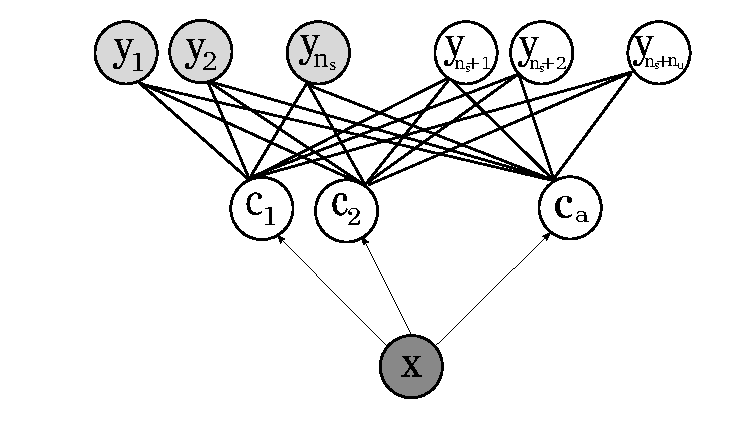
\includegraphics[width=\linewidth]{images/dap}
    \caption{}
    \label{fig:dap}
  \end{subfigure}
%
  \begin{subfigure}[b]{0.47\linewidth}
    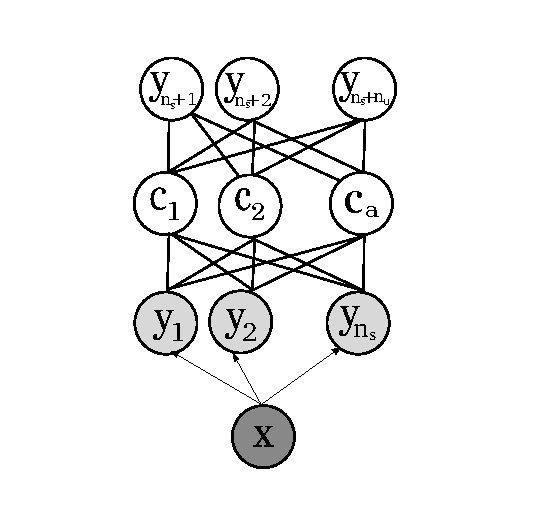
\includegraphics[width=\linewidth]{images/iap}
    \caption{}
% \caption{Points colored according to their ground truth labels}
    \label{fig:iap}
  \end{subfigure}
  \caption[مدل گرافی پیش‌بینی ویژگی مستقیم و غیرمستقیم]{
  مدل گرافی پیش‌بینی ویژگی مستقیم (آ) و غیر مستقیم (ب). رئوس با سایه‌ی روشن رئوسی هستند که در زمان آموزش رویت شده هستند و رئوس با سایه‌ی تیره همواره رویت شده‌اند. رئوس بدون سایه مربوط به متغیرهایی است که باید استنتاج در مورد آن‌ها انجام شود. یال‌های ضخیم‌تر روابط ثابت را نشان می‌دهند که جزو داده‌های آموزش هستند و یال‌های نازک‌تر روابطی را که باید کشف شوند. $x$ یک تصویر است، متغیرهای دودویی
  $y_1, \ldots y_{n_s}$
  تعلق یا عدم تعلق تصویر به دسته‌های دیده شده و بصورت مشابه 
  $y_{n_s +1}, \ldots y_{n_s+n_u}$
  تعلق یا عدم تعلق به دسته‌های دیده نشده را نشان می‌دهند. 
  $c_1, \ldots, c_a$
  ویژگی‌های توصیف‌کننده دسته‌ها هستند.
\textbf{آ)}
در مدل پیش‌بینی ویژگی مستقیم رابطه میان برچسب‌ها و ویژگی‌ها ثابت فرض می‌شود و هدف استنتاج ویژگی از روی تصاویر است. بعد از آن با استفاده از رابطه از پیش تعیین شده برچسب‌ها با ویژگی‌ها، برچسب تعیین می‌شود. 
\textbf{ب)}
در مدل پیش‌بینی ویژگی غیر مستقیم، یک دسته‌بند چنددسته‌ای روی دسته‌های آموزش یادگرفته می‌شود و با توجه به وقوع یا عدم وقوع هر یک از ویژگی‌ها در این دسته‌ها رابطه‌ی ثابتی میان دسته‌های دیده شده 
$y_1, \ldots y_{n_s}$
و ویژگی‌ها فرض می‌شود. هم‌چنین رابطه ویژگی‌ها با دسته‌های دیده نشده 
$y_{n_s +1}, \ldots y_{n_s+n_u}$
رابطه امضا بودن است و دانسته فرض می‌شود \cite{lampert09}.
  }
  \label{fig:diap}
\end{figure}

در \cite{hinton09} از چند رگرسیون منطقی\LTRfootnote{Logistic Regression}  مستقل برای پیش‌بینی‌های ویژگی دودویی از تصاویر \lr{fMRI} استفاده شده و سپس دسته‌بندی با دسته‌بند نزدیک‌ترین همسایه بر اساس نزدیکی بردار ویژگی پیش‌بینی شده و امضای دسته‌های آزمون صورت می‌پذیرد.

در
\cite{lampert09}
با فرض این که ویژگی‌ها به صورت مستقل از یکدیگر قابل پیش‌بینی هستند دو رویکرد برای این کار ارائه می‌کند. پیش‌بینی ویژگی مستقیم\LTRfootnote{Direct Attribute Prediction}
و پیش‌بینی ویژگی غیر مستقیم\LTRfootnote{Indirect Attribute Prediction}.
 مدل گرافی مورد استفاده در این دو رویکرد در تصویر \ref{fig:diap} آمده است. در پیش‌بینی ویژگی مستقیم برچسب‌ها به شرط دانستن ویژگی‌های درون تصویر، از تصویر مستقل هستند. در این روش برای هر یک ویژگی‌ها یک دسته‌بند یاد گرفته می‌شود. با توجه به این که ویژگی‌ها برای تصاویر آزمون معین هستند این کار با استفاده از یک دسته‌بند احتمالی برای هر ویژگی قابل انجام است. در نهایت احتمال تعلق هر یک از برچسب‌های
$ u \in \mathcal{U} $
با استفاده از رابطه زیر بدست خواهد آمد.
\begin{equation} \label{eq:dap0}
  P(u | \mathbf{x}  ) = \sum_{\mathbf{c} \in \{0,1\}^a} P(u | \mathbf{x} ) p(\mathbf{c} |\mathbf{x} )
\end{equation}
از با توجه به فرض استقلال ویژگی داریم
$P(\mathbf{c} |\mathbf{x} ) = \prod_{n=1}^a P(\mathbf{c} _m |\mathbf{x} )$.
برای محاسبه جمله 
$P(u | \mathbf{c} )$ 
از قانون بیز استفاده می‌کنیم:
\[
P(\mathbf{u}  | \mathbf{c} ) = \frac{P(u)P(\mathbf{c} |u)}{P(\mathbf{c_u} )}  = \frac {P(u) \mathds{1}(c= \mathbf{c_u} )} {P(\mathbf{c_u} )}
\]
با جایگذاری در رابطه \eqref{eq:dap0} خواهیم داشت:
\begin{equation}
  P(u | \mathbf{x}  ) = \frac{P(u)}{P(\mathbf{c_u} )} \prod_{n=1}^a P(\mathbf{c}_{\mathbf{u} n}|\mathbf{x} )
\end{equation}
در نهایت برچسبی که احتمال فوق را بیشینه کند، پیش‌بینی مربوط به تصویر $x$ خواهد بود.

در روش پیش‌بینی ویژگی غیر مستقیم، IAP
 تخمین  $P(c_i|\mathbf{x}) $ تغییر داده می‌شود؛ به این صورت که ابتدا یک دسته‌بند چند دسته‌ای یعنی $P(y_k |\mathbf{x})$ روی داده‌ها یاد گرفته می‌شود و سپس رابطه ویژگی‌ها و برچسب‌ها به صورت قطعی مدل می‌شود:
\begin{equation}
P(\mathbf{c}_i | \mathbf{x}) = \sum_{k=1}^{n_u} P(y_k | \mathbf{x}) \mathbb{I}(\mathbf{c}_i = \mathbf{c}_{\mathbf{y_k}i})
\end{equation}
در نهایت در هر دو روش برچسب نهایی با تخمین MAP\LTRfootnote{Maximum a Posteriori}
از رابطه زیر تعیین می‌شود:
\begin{equation}
\hat{y} = \argmax_{u \in \mathcal{U}} P(u|\mathbf{x}) =  \argmax_{u \in \mathcal{U}} \prod_{i=1}^a \frac{P(\mathbf{c}_{\mathbf{u}i} | \mathbf{x})}{P(\mathbf{c}_{\mathbf{u}i})}
\end{equation}
روش ارائه شده در
\cite{suzuki14}
مشابه همین روش است با این تفاوت که احتمال مشاهده هر کدام ویژگی‌ها را هم در محاسبه دخیل می‌کند تا با وزن‌های متفاوت با توجه به اهمیتشان در دسته‌بندی نقش داشته باشند. ضعف بزرگ این روش‌ها فرض مستقل بودن ویژگی‌ها از یکدیگر است؛ چرا که این فرض در مسائل واقعی معمولا بر قرار نیست. برای مثال زمانی که ویژگی آبزی بودن برای یک موجود در نظر گرفته می‌شود احتمال ویژگی پرواز کردن برای آن بسیار کاهش می‌یابد.
\subsection{مدل‌سازی احتمالی روابط بین ویژگی‌ها}
مدل‌های گرافی برای در نظر گرفتن وابستگی‌های میان ویژگی‌ها به کار گرفته شده‌اند. نویسندگان \cite{topicmodel} برای در نظر گرفتن ارتباط بین ویژگی‌ها و ارتباط ویژگی‌ها با برچسب نهایی روش‌های مدل‌سازی موضوع \LTRfootnote{  Topic Modeling} را از حوزه یادگیری در متن اقتباس می‌کنند. همچنین  نویسندگان \cite{unified13} برای این کار یک چارچوب بر اساس مدل‌های گرافی احتمال معرفی می‌کنند. در این چارچوب یک شبکه بیزی\LTRfootnote{  Baysian Network}  برای مدل کردن این روابط در نظر گرفته می‌شود و ساختار آن که نشان‌دهنده وابستگی یا استقلال ویژگی‌ها با هم یا با برچسب است، با کمک روش‌های یادگیری ساختار\LTRfootnote{Structure Learning}
شناخته می‌شود.

\section{نگاشت به فضای توصیف‌ها}
در برخی موارد توصیف‌های داده شده از جنسی غیر از ویژگی هستند ولی فضای مشترک همان فضای توصیف‌ها در نظر گرفته می‌شود و سعی می‌شود تصاویر به این فضا نگاشته شوند.
%------------------------------------------ConSE
روش ConSE\LTRfootnote{Convex combination of Semantic Embeddings}
 \cite{convex} 
از چنین نگاشتی استفاده می‌کند.  ابتدا یک شبکه عصبی کانولوشنال برای دسته‌بندی نمونه‌های دسته‌های دیده‌شده آموزش داده می‌شود. این یادگیری یک مسئله دسته‌بندی عادی است و شبکه‌ها در اکثر موارد از قبل به صورت پیش‌آموزش دیده شده وجود دارند. تابع فعال‌سازی\LTRfootnote{Activation Function} 
  لایه‌ی آخر این شبکه  به این صورت تعریف می‌شود:
 \begin{equation}
 \label{softmax}
 softmax(z)_j = \frac{e^{z_j}}{\sum_k e^{z_k}}, \quad j = 1, \ldots, n_s.
 \end{equation} 
 تابع بالا به ازای هر $j$، امتیاز تعلق نمونه به دسته‌ی $j$م را نشان می‌دهد. در هنگامی که با مسئله دسته‌بندی عادی روبرو هستیم، روی $j$ بیشینه گرفته می‌شود و دسته‌ای که بیشترین امتیاز را گرفته به عنوان پیش‌بینی خروجی داده می‌شود. در روش ConSE برای مسئله یادگیری بدون برد، هنگامی که یک نمونه از دسته‌های آزمون را به شبکه می‌دهیم، خروجی بدست آمده از رابطه \eqref{softmax} می‌تواند به عنوان میزان شباهت آن نمونه به هر یک دسته‌های آموزش در نظر گرفته شود. 
  فرض کنید که برای هر نمونه
 $\hat{y}(x,n)$،
 $n$مین 
 عنصر بزرگ $softmax(x)$ را نشان دهد، یعنی $n$مین برچسب محتمل برای $x$ از میان دسته‌های آموزش. حالا برای پیش‌بینی برچسب $x$ از میان دسته‌های آموزش از این رابطه استفاده می‌کنیم:
 \begin{equation}
 \label{eq:conse}
 \phi(x) = \frac{1}{Z} \sum_{n=1}^T P(\hat{y}(x,n) | x) \cdot c_{\hat{y}(x,n)},
 \end{equation}
 که $T$ یک فراپارامتر مدل
 $Z = \sum_{n=1}^T P(\hat{y}(x,n) | x) $
 ضریب نرمال‌سازی است. در این حالت نمونه‌ی $x$ با تابع $\phi(\cdot)$ به فضای توصیف‌ها نگاشته شده است. به عبارت دقیق‌تر به صورت جمع وزن‌دار توصیف $T$ دسته‌ی شبیه‌تر نمایش داده شده است که وزن‌های این جمع میزان شباهت هستند. 
 % COSTA -----------------------------------------Extendtable
 روش \lr{COSTA}\LTRfootnote{Co-Occurance Statistics}
 \cite{costa}
 نیز از رویکرد مشابهی استفاده می‌کند. در این روش همانند رابطه \eqref{eq:conse}، پارامترهای دسته‌بند برای دسته‌های دیده نشده به صورت جمع وزن‌دار پارامترهای دسته‌بندهای دسته‌های دیده شده بیان می‌گردد. در این پژوهش برای بدست آوردن وزن‌های مربوط به شباهت میان دسته‌ها توابع مختلفی از تعداد رخ‌داد همزمان برچسب‌ها پیشنهاد شده است.




%----------------------------Bilinear maps 
\section{نگاشت‌های دو خطی}
حالت دیگری از چارچوب کلی معرفی شده در ابتدای فصل این است که نگاشت به فضای مشترک یک نگاشت دوخطی باشد. یعنی به این صورت که $W$ نگاشتی خطی است که $x^TW$ تصویر $x$ را به فضای توصیف‌ها نگاشته و $Wc$ توصیف $c$ را به فضای تصاویر می‌نگارد.در نهایت تابع مطابقت میان یک توصیف و تصویر به صورت زیر تعریف می‌شود:
\begin{equation}\label{bilinear}
F(x,c) = \phi(x)^TW \theta(y)
\end{equation}
 در این حالت، این که فضای مشترک در حقیقت کدام یک از فضاهای تصاویر یا توصیفات هستند، جواب روشنی ندارد. نقطه‌ی قوت این روش‌ها در امکان پیچیده‌تر کردن تابع هزینه است. چرا که در حالتی که نگاشت خطی است مسائل بهینه‌سازی پیچیده‌تری نسبت به حالت غیر خطی قابل حل خواهند بود.

 \subsection{یادگیری با توابع رتبه‌بند}
  یک انتخاب متداول برای تابع هزینه، توابع رتبه‌بند\LTRfootnote{ranking function}
هستند. با توجه به این که عموما بعد از یادگیری این نگاشت، دسته‌ای که نزدیک‌ترین توصیف را (با معیاری مثل فاصله یا ضرب داخلی) دارد، به عنوان پیش‌بینی تولید می‌شود،
 چنین تابع هزینه‌ای یک انتخاب طبیعی است. چرا که مسئله‌ی نزدیکترین همسایه در اصل یک مسئله رتبه‌بندی
 است و استفاده از یک تابع هزینه‌ی رتبه‌بند برای یادیگری نگاشت بهتر از مجموع مربعات است که تنها فاصله نقاط از برچسب خودشان را در نظر می‌گیرد \cite{devise}.

در
\cite{akata2013}
 تابع هزینه رتبه‌بند WSABIE
\cite{wsabie}
که برای حاشیه‌نویسی تصاویر پیشنهاد شده، به مسئله یادگیری بدون برد انطباق می‌دهد.
تابع هزینه WSABIE به این صورت تعریف شده است:

\begin{align}
L(x_s, Y_s ; W, \theta) = \frac{1}{N_s} \sum_{n=1}^{N_s} \lambda_{r_\Delta (x_n, y_n)} \sum_{y \in \mathcal{Y}} \max (0, \mathit{l}(x_n, y_n, y) ) \\
\mathit{l}(x_n,y_n,y) = \mathds{1}(y \neq y_n) + \phi(x_n)^TW \theta(y) - \phi(x_n)^TW\theta(y_n) \label{l_loss}
\end{align}

که در آن
$ r_\Delta (x_n, y_n) =  \sum_{y \in \mathcal{Y}} \mathbb{I}(\mathit{l}(x_n, y_n, y)  > 0) $
 و $\lambda_k$ یک تابع نزولی از $k$ است. این تابع، پیش‌بینی اشتباه ویژگی‌ها را  این گونه جریمه می‌کند که به ازای برچسب نادرستی که رتبه بالاتری از برچسب صحیح در دسته‌بندی دریافت کرده، جریمه‌ای متناسب با امتیاز برچسب ناصحیح در نظر گرفته می‌شود.ضریب نزولی $\lambda_k$ میزان جریمه را برای برچسب‌های غلط در رتبه‌های بالا، بیشتر در نظر می‌گیرد. در انطباق برای یادگیری بدون برد، بهینه‌سازی تنها روی نگاشت $W$ انجام شده و  تابع $\theta$ دانسته فرض می‌شود:
$\theta(y) = c_y$.


ایده‌ی بالا در \cite{Akata2015} ادامه داده شده و نگاشت شباهت ساخت‌یافته
\lr{SJE}\LTRfootnote{Structured Joint Embedding}
نامیده شده است.
، در این حالت تابع مطابقت بین توصیف‌ها و تصاویر از رابطه  \eqref{bilinear} تعریف می‌شود. تابع هزینه ساده‌تر از حالت قبل به صورت
\begin{equation} \label{sje_loss}
\frac{1}{N_s} \sum_{n=1}^{N_s} \max_{y \in \mathcal{Y}}(0, l(x_n, y_n, y))
\end{equation}
در نظر گرفته شده که $l$ همانند رابطه \eqref{l_loss} است. هم‌چنین برای استفاده از چند توصیف به صورت هم‌زمان، تعریف تابع مطابقت به صورت زیر تعمیم داده می‌شود:
\begin{align}
F(x,y;\{W\}_{1\ldots K}) &= \sum_k \alpha_k \theta(x)^T W_k \phi_k(y)  \\
s.t. & \sum_k \alpha_k = 1 \nonumber
\end{align}
که $\phi_k(y)$ توصیف‌های مختلف از دسته‌ی $y$ را نشان می‌دهد و $W_1, \ldots W_K$ نگاشت‌های میان هر یک از این توصیف‌ها و فضای تصاویر را. وزن‌های $\alpha_k$ که میزان اهمیت یا اطمینان  هر یک از توصیف‌ها را نشان می‌دهد، با اعتبارسنجی تعیین می‌شوند. روش \lr{SJE} با انواع اطلاعات جانبی سازگار است. اطلاعات جانبی که بر روی آن‌ها تست انجام شده است شامل بردار ویژگی‌های دودویی یا پیوسته تعیین شده توسط انسان و نمایش برداری متون دائره‌المعارفی با روش‌های \lr{word2vec} \cite{word2vec} و GloVe
\cite{pennington2014glove}
است. هم‌چنین نویسندگان این پژوهش یک نسخه با نظارت از \lr{word2vec} ارائه می‌دهند که در جریان آموزش آن از موضوع هر متن هم استفاده می‌شود.

 روش \lr{SJE} در \cite{Xian2016} برای برخی نگاشت‌های غیرخطی نیز تعمیم داده شده است. در این روش  که
 \lr{LatEm}\LTRfootnote{Latent Embedding Model}
 نام دارد تابع هزینه مانند حالت قبل (رابطه \eqref{sje_loss}) تعریف شده است با این تفاوت که تابع مطابقت میان توصیف و تصویر بجای رابطه دوخطی \eqref{bilinear} از این رابطه تبعیت می‌کند:
 \begin{equation} \label{latem}
 F(x,y) = \max_{1\leq i \leq L} \phi(x)^TW \theta(y)
 \end{equation}
در این حالت تابع مطابقت به صورت ترکیب نگاشت‌های دوخطی $W_1, \ldots W_M$ بیان شده است و یک تابع غیر خطی ولی تکه‌تکه خطی برای تصمیم‌گیری مورد استفاده قرار می‌گیرد.

یک تعمیم دیگر از SJE در \cite{multicue} ارائه شده است که در آن فرض وجود اطلاعات نظارتی قوی‌تر در نظر گرفته شده است.  در این حالت فرض می‌شود که در تصاویر قسمت‌های مختلفی که توصیفی از آن‌ها موجود است، مشخص شده‌اند. البته تناظر میان قسمت‌های توصیف و تصویر موجود نیست، مثلا در مجموعه دادگان مربوط به پرنده‌ها، قسمت‌های مختلف بدن پرنده مانند نوک و پا در همه تصاویر جدا شده است اما این اطلاعات که هر کدام از این‌ها به چه قسمتی از توصیف آن دسته مربوط می‌شوند، در دسترس نیست. با این فرض تابع مطابقت $F$ تعریف شده در رابطه \eqref{bilinear} به گونه‌ای تعمیم داده می‌شود که مطابقت قسمت‌های مختلف متن و تصویر را بسنجد:
\begin{align}
F(x,y) = \frac{1}{|g_x||g_y|} \sum_{i\in g_x}\sum_{j\in g_y} \max(0,v_i^Ts_j),
\end{align}
که در آن 
 $g_x$ 
 مجموعه قسمت‌های مختلف تصویر $x$ و  $g_y$ مجموعه قسمت‌های توصیف ارائه شده‌ی دسته‌ی $y$ است. $s_j$ و $v_i$ که به ترتیب بازنمایی یک قسمت از متن و تصویر هستند به صورت زیر تعریف می‌شوند:
 
\begin{align}
& s_j = f\left( \sum_m W^{\text{language}}_m l_m + b^{\text{language}} \right) \nonumber \\
& v_i = W^\text{visual} [CNN_{\theta_c}(I_b)] + b^{\text{visual}}.
\end{align}
$l_m$
انوع مختلف توصیف را نشان می‌دهند که در این پژوهش شامل بردار ویژگی، نمایش \lr{word2vec}  و کیسه‌ی کلمات متون توصیف کننده است. در نهایت یادگیری این پارامترها با تابع هزینه‌ی بیشترین حاشیه انجام می‌شود.


در
\cite{devise}
نیز که برای اولین بار توصیف تنها نام برچسب دسته‌ها در نظر گرفته شده، از نگاشت دو خطی استفاده شده است. در این روش نام برچسب‌ها با استفاده از مدل نهان‌سازی کلمات \lr{word2vec} کلمات به بردارهایی نگاشته می‌شوند. ابعاد فضای نهان‌سازی کلمات یک فراپارامتر است که در این مقاله با اعتبار سنجی تعیین شده است. استخراج ویژگی از  تصاویر  با استفاده از شبکه عصبی کانولوشنال
\cite{alexnet}
که روی دسته‌های دیده شده آموزش داده شده، انجام می‌شود. در نهایت یک تابع بیشترین حاشیه\LTRfootnote{Max margin}
برای یادگیری نگاشت دو خطی پیشنهاد می‌شود.
\begin{equation}
 L((x_n, y_n);W) = \sum_{y\neq y_n} \max(0, \xi  - x_nWc_{y_n} + x_nWc_y)
\end{equation}
که در آن $\xi$ حاشیه دسته‌بندی است. دسته‌بندی نمونه‌های جدید با نگاشتن $x$ به فضای برچسب‌ها و استفاده از دسته‌بند نزدیکترین همسایه صورت می‌گیرد.

\subsection{روش‌های مبتنی بر خطای مجموع مربعات} \label{mse_loss_methods}

%-------------------------------------------- EZSL ----------------------------------------------------------------------------------
یک نحوه‌ی استفاده دیگر از نگاشت‌های دو خطی، دسته‌بندی مستقیم با این نگاشت است.
\begin{equation}
\minimize_{W \in \mathbb{R}^{d \times a}} \normf{X_s^T WC_s - Y} + \Omega(W) \label{eq:emb}
\end{equation}
که در آن $\Omega$ یک جمله منظم‌سازی است.
در این حالت اگر تبدیل را از فضای تصاویر به فضای ویژگی‌ها نگاه کنیم، نگاشت $W$ باید تصاویر را به زیرفضایی عمود به تمامی بردار ویژگی‌های مربوط به برچسب‌های نادرست بنگارد.
عملکرد خوب این روش، با وجود استفاده از تابع هزینه ساده مجموع مربعات خطا که در یادگیری ماشین تابع هزینه‌ی مناسبی برای دسته‌بندی به شمار نمی‌آید، به جمله منظم سازی آن نسبت داده می‌شود. جمله منظم‌سازی $\Omega$ به این صورت تعریف می‌شود:
\begin{equation} \label{eq:emb_reg}
\Omega(W) = \lambda \normf{WC_s} + \gamma \normf{X_s^T W}  + \lambda \gamma \normf{W}
\end{equation}
این جمله منظم‌سازی با دیدگاه نگاشت دوخطی طبیعی است. چرا که ماتریس $WC_S$ را می‌توان یک دسته‌بند خطی روی فضای تصاویر در نظر گرفت و از طرفی ماتریس $X_s^T W$ یک دسته‌بند روی بردارهای ویژگی است در نتیجه طبیعی است که پارامترهای این دو دسته‌بند با نرم فروبنیوس آن‌ها کنترل شود تا از بیش‌‌برازش\LTRfootnote{overfitting}
 جلوگیری شود.
استفاده از توابع نرم دوم برای خطا و منظم‌سازی در این روش باعث شده است که مسئله بهینه‌سازی جواب به صورت فرم بسته داشته باشد و زمان اجرا نسبت به سایر روش‌ها بسیار کمتر باشد.

%----------------------------------------------------------------------------LESS IS MORE
این روش در
\cite{lessismore}
برای توصیفات متنی توسعه داده شده است. با توجه به ابعاد بالای داده‌های متنی و همچنین نویز زیادی که در آن‌ها در مقایسه با بردارهای ویژگی وجود دارد، ماتریس تبدیل $W$ به دو ماتریس تجزیه می‌شود:
\begin{equation}
W = V_x^T V_c
\end{equation}
با این تجزیه از افزایش شدید تعداد پارامترها در اثر افزایش بعد بردار توصیف‌ها جلوگیری می‌شود. (دقت کنید که بعد $C$ برابر $d\times a$ است) علاوه بر این $V_c$ می‌تواند برای استخراج ویژگی‌های مفید و حذف نویز از  $C$ به  کار گرفته شود و $V_x$ مانند $W$ در حالت اصلی عمل کند یعنی پارامترهای یک دسته‌بند را از روی توصیف‌ها تولید کند. در نهایت تابع هزینه برای این روش به صورت زیر تعریف می‌شود:
\begin{equation}
\min_{V_x, V_c} \normf{X_s^T + V_x^T V_c C} + \lambda_1 \normf{ V_x^T V_c C} +
\lambda_2 \norm{V_c^T}_{2,1}
\end{equation}
که
$\norm{M^T}_{2,1} = \sum_i \norm{M_{(i)}}_2 $
و این نوع منظم‌سازی، ستون‌های ماتریس $V_c$ را به سمت تنک بودن سوق خواهد داد. در واقع اگر $\lambda_2$ بزرگ انتخاب شود، $V_c$ نقش یک ماتریس انتخاب ویژگی\LTRfootnote{feature selection}
را خواهد داشت. جمله‌های منظم سازی دیگر در
\eqref{eq:emb_reg}
به دلیل تاثیر اندکشان در آزمایشات عملی حذف شده‌اند.


\section{نگاشت به فضای تصاویر}\label{to_images}
در برخی از روش‌ها فضای مشترک فضای ویژگی‌های تصویر است و نگاشتی از توصیف‌ها به این فضا یاد گرفته می‌شود و مطابقت تصویر و توصیف در این فضا قابل سنجیدن می‌شود. از آن‌جا که در این روش‌‌ها، استخراج ویژگی از تصاویر با توابع از پیش معین صورت می‌گیرد این روش‌ها را با عنوان نگاشت به فضای تصاویر بررسی می‌کنیم.


 یک تعمیم  از \lr{SJE} در \cite{Reed2016} ارائه شده است. در این روش که برای تصاویر مجموعه متون بزرگتری نسبت به دادگان قبلی جمع‌آوری و استفاده شده است.
  این ازدیاد در داده‌ها امکان آموزش مدل‌های پیچیده‌تر و پیشرفته‌تر را برای یادگیری نگاشت از فضای تصاویر فراهم می‌کند و فاصله میان عمل‌کرد یادگیری بدون برد هنگام استفاده از
  توصیف‌های متنی و توصیف‌های به صورت بردار ویژگی را کمتر کرده است.
  در این حالت فرض می‌شود که داده‌های آموزش به صورت
   $\{(v_{n},t_{n},y_{n}), n = 1, ..., N\}$
   است که متشکل است از
    $v \in \mathcal{V}$
    که ویژگی‌های تصویری هستند،
     $t \in \mathcal{T}$ توصیفات متنی و $y \in \mathcal{Y}$ برچسب‌ها.
      دقت کنید که در توصیف این روش بر خلاف سایر روش‌ها از نمادگذاری معرفی شده در این بخش استفاده نکرده‌ایم.
      نمادهای استفاده شده منطبق بر نمادهای مقاله اصلی می‌باشند. دلیل این موضوع این است که ویژگی‌های تصویری $v_n$ با با تصاویر  $x_n$ متفاوت است. در نمادگذاری ما هر $x$ در رابطه یک‌به‌یک با یک تصویر آموزش یا آزمون است در حالی‌که در مجموعه آموزش معرفی‌شده در بالا هر تصویر با چند مجوعه ویژگی بصری $v$ در مجموعه آموزش حضور دارد و هر کدام از این ويژگی‌های بصری $v_n$، یک متن مربوط به خود دارد که با $t_n$ نشان داده ‌شده است. هم‌چنین فرض کنید که  $\mathcal{T}(y)$ و $\mathcal{V}(y)$ به ترتیب مجموعه تمامی متون و ویژگی‌های بصری مربوط به کلاس $y$ را نشان می‌دهند.
  در این حالت هدف یادگیری تابع مطابقت $F : \mathcal{V} \times \mathcal{T} \rightarrow \mathbb{R}$ میان تصاویر و توصیف‌هاست. که به صورت
  \begin{equation}
  \label{eq:akata16comp}
F(v, t) = \theta(v)^T\phi(t)
  \end{equation}
در نظر گرفته شده است. با داشتن چنین تابعی، مشابه سایر روش‌ها پیش‌بنی برچسب برای تصاویر یا حتی متون جدید با معادلات زیر صورت می‌پذیرد:
\begin{align}
\label{eq:akata16class}
f_v(v) = \underset{y \in \mathcal{Y}}\argmax ( \mathbb{ E}_{t \sim \mathcal{T}(y)}[F(v, t)])\\
f_t(t) = \underset{y \in \mathcal{Y}}\argmax (\mathbb{ E}_{v \sim \mathcal{V}(y)}[F(v, t)]).
\end{align}
یادگیری تابع $F$ با تابع هزینه‌ی زیر صورت می‌گیرد:
\begin{align}
\label{eq:objective_actual}
\dfrac{1}{N}\sum_{n=1}^{N} \ell_v(v_n, t_n, y_n) + \ell_t(v_n, t_n, y_n),
\end{align}
که توابع $ \ell_t$ و $\ell_v$ این گونه تعریف شده اند:
\begin{align*}
\ell_v(v_n, t_n, y_n) &=  \underset{y \in \mathcal{Y}}{\max}(0,\Delta(y_n, y) + \mathbb{E}_{t \sim \mathcal{T}(y)} [ F(v_n,t) - F(v_n,t_n) ]) \\
\ell_t(v_n, t_n, y_n) &= \underset{y \in \mathcal{Y}}{\max}(0,\Delta(y_n, y) + \mathbb{E}_{v \sim \mathcal{V}(y)} [ F(v,t_n) - F(v_n,t_n)])
\end{align*}
تفاوت این تابع هزینه با  رابطه \eqref{sje_loss} در اضافه شدن جمله‌ی دوم است. در  رابطه \eqref{sje_loss} این مسئله که هر تصویر طوری نگاشته شود که به توصیف درست نزدیک‌تر از بقیه توصیف‌ها باشد در نظر گرفته می‌شد، در رابطه بالا علاوه به این مسئله، نگاشت‌ها باید طوری باشد که هر توصیف باید به ويژگی بصری خود نزدیک‌تر باشد تا سایر ویژگی‌های بصری.
نگاشت $\theta$ مانند سایر روش‌ها یک شبکه عصبی عمیق کانولوشنال است که از قبل با داده‌های \lr{ImageNet} آموزش داده شدهاست. برای هر تصویر قسمت‌های بصری مختلف با بریدن قسمت‌های متفاوت از تصویر حاصل می‌شود. نگاشت $\phi$ برای متون با سه شبکه عصبی مختلق کانولوشنال، بازگردنده و کانولوشنال بازگردنده\lr{ (CNN-RNN) } مدل شده است. استفاده از این شبکه‌ها برای نگاشت متن در این روش نخستین بار در این روش رخ داده‌است. جمع‌آوری مجموعه دادگان متنی بزرگتر، آموزش چنین شبکه‌هایی را ممکن کرده است.

در  \cite{mohamed13} که برای نخستین بار توصیف‌ها از نوع متنی مورد بررسی قرار گرفته شده است، راه‌حل پیشنهادی یادگیری نگاشتی از این توصیفات به فضای تصاویر است. حاصل این نگاشت یک دسته‌بند خطی در فضای تصاویر در نظر گرفته می‌شود. اگر این نگاشت را طبق نمادگذاری معرفی شده با $\phi$ نشان دهیم دسته بندی با استفاده از رابطه زیر انجام خواهد شد:
\begin{equation} \label{eq:linear_classifier}
y^* = \argmax_y \phi(c^y)^T x
\end{equation}


برای یادگیری $\phi(c)$ از ترکیب دو تخمین‌گر استفاده می‌شود:
\begin{enumerate}
\item
رگرسیون احتمالی: توزیع $P_{reg}$ یادگرفته می‌شود که برای یک توصیف $c$ و نگاشت در فضای تصاویر $w$ احتمال $P_{reg}(w|c)$ را مدل می‌کند.
\item
تابع مطابقت: نگاشت دو خطی $D$ که تطابق میان دامنه تصاویر و توصیف‌ها مدل می‌کند به عبارت دیگر $c^TDx$ زمانی که $x$ به دسته‌ای که   $c$ توصیف می‌کند تعلق دارد بزرگتر از مقدار آستانه‌ای است و در غیر این صورت کوچک‌تر از آن. می‌توان مشاهده کرد که در این حالت با استفاده از رابطه
\eqref{eq:linear_classifier}،
 $c^TW$
یک  دسته‌بند خطی برای دسته‌ای که $c$ توصیف می‌کند، خواهد بود.
\end{enumerate}

پارامترهای $P_{reg}$ و $D$ با استفاده از نمونه‌های آموزش بدست می‌آیند.
در نهایت تابع پیشنهادی برای نگاشت $\phi$ برای دسته‌های آزمون به صورت زیر تعریف می‌شود:
\begin{align}
\label{eq:write_a}
\phi(c) &= \argmin_{w,\zeta_i} w^Tw - \alpha c^TDw -\beta \, ln(P_{reg}(w|c)) + \gamma \sum \zeta_i \\
s.t. \, &: -(w^tx_i) \geq \zeta_i, \quad \zeta_i \geq 0, \, i=1,\ldots N_s  \nonumber \\
& c^TDc \geq l \nonumber
\end{align}
که $\alpha, \beta, \gamma, l$ فراپارامترهای مدل هستند. جمله اول در این تابع هزینه، منظم‌سازی دسته‌بند خطی $w$ است. جمله دوم مشابهت $w$ با $c^TD$ را الزام می‌کند و جمله سوم احتمال بالا در رگرسیون را در نظر می‌گیرد. محدودیت $-(w^Tx_i) \geq \zeta_i$ بر اساس فرض عدم تعلق
نمونه‌های آزمون به کلاس‌های دیده‌شده تعریف شده است و اجبار می‌کند که تمامی نمونه‌های دیده‌شده باید در طرف منفی دسته‌بند خطی $w$ قرار گیرند.
نویسندگان این پژوهش، روش خود را با استفاده از تکنیک هسته
\LTRfootnote{kernel trick}
برای دسته‌بندهای غیرخطی نیز توسعه داده‌اند \cite{elhoseiny2015}.

\section{نگاشت به یک فضای میانی}
در برخی روش‌ها هر دوی نگاشت‌های $\phi$ و $\theta$، معرفی شده در ابتدای فصل با توجه به داده‌ها یاد گرفته می‌شوند و در نتیجه فضای مشترک مورد استفاده نه فضای تصاویر و نه فضای توصیف‌هاست؛ بلکه فضای ثالثی است. این فضای میانی در برخی از روش‌ها یک فضای با بعد کمتر است و تعبیر معنایی برای آن موجود نیست. در برخی روش‌های دیگر، فضای میانی را با بعد $n_s$ یعنی تعداد دسته‌های دیده شده در نظر گرفته‌اند و تعبیر معنایی برای آن ارائه شده است. این فضای میانی بر اساس توصیف دسته‌ها و نمونه‌های دیده نشده بر اساس شباهت آن‌ها با دسته‌های دیده شده استوار است.

%-------------predicting salakhudtinov
\begin{figure}[th] 
\begin{center}
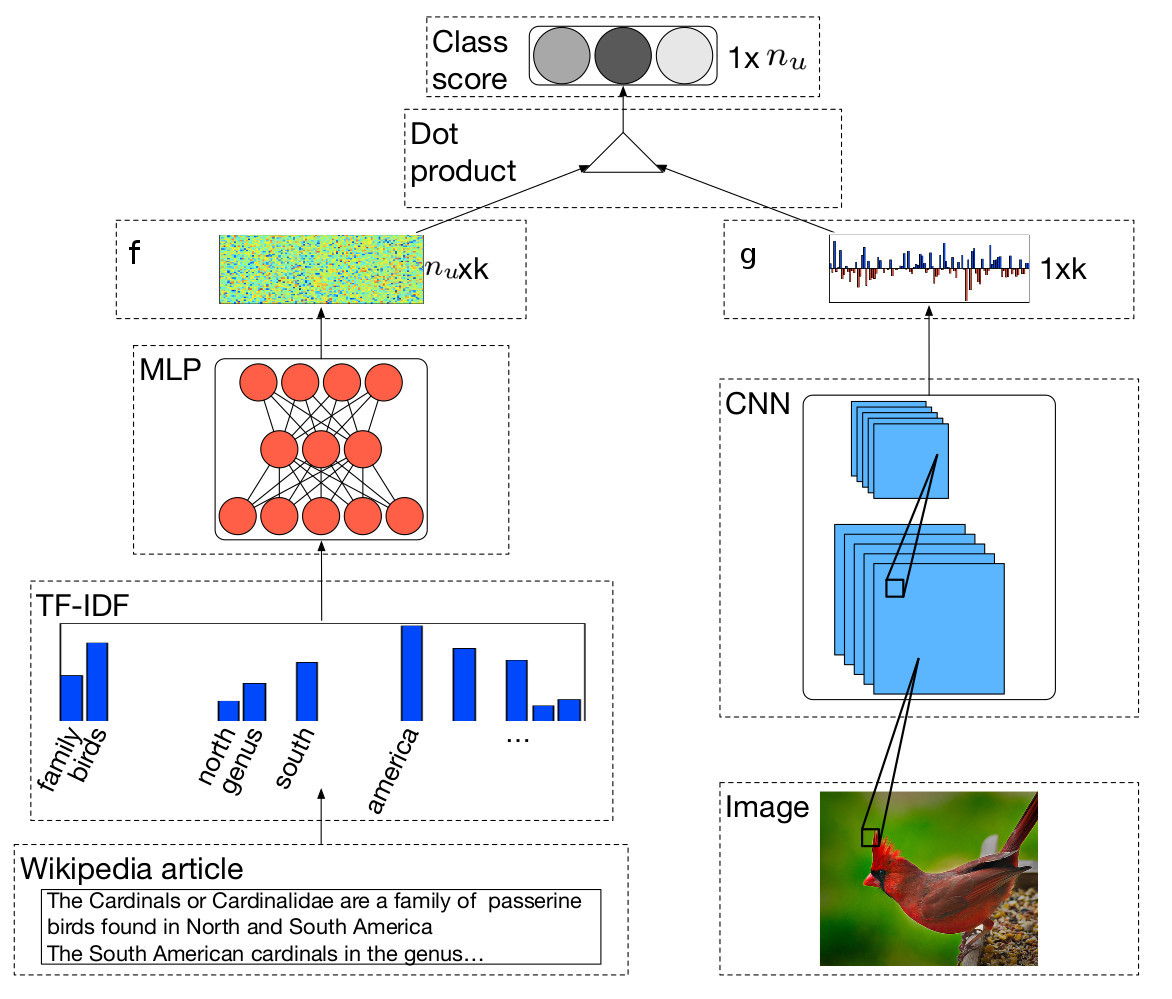
\includegraphics[width=7cm]{images/ba.jpg}
\end{center}
\caption[نمای کلی روش \cite{ba2015}]{
 شبکه مورد استفاده برای یادگیری توام نگاشت تصاویر و توصیف‌ها که یک شبکه عصبی عمیق با دو ورودی است. ورودی اول از نوع تصویر است و ابتدا با یک شبکه کانولوشنال سپس با چند لایه چگال به فضایی $k-$بعدی می‌رود. ورودی دوم که یک مقاله از ویکی‌پدیای انلگیسی است پس از تبدیل به نماش برداری به صورت \lr{tf-idf} با چندلایه با اتصالات چگال پردازش شده و به فضایی $k-$بعدی می‌رود. در نهایت امتیاز تعلق تصویر به دسته‌ی متن با ضرب داخلی این دو نگاشت تعیین می‌شود \cite{ba2015}.
}
\label{fig:deep}
\end{figure}

در  \cite{ba2015} از شبکه‌های عصبی عمیق برای یادگیری توام نگاشت‌های $\phi$ و $\theta$ استفاده شده است. نمای کلی شبکه مورد استفاده در این روش در تصویر
\ref{fig:deep}
نشان داده شده است. توصیف‌های متنی و ويژگی‌های بصری دو ورودی جداگانه به چنین شبکه‌ای هستند که ابتدا به صورت جداگانه با یک یا چند لایه‌ی با اتصالات کامل به یک فضای مشترک نگاشته شده و سپس بر اساس شباهت نمایش آن‌ها در این فضای میانی دسته‌بندی می‌شوند. تفاوت این روش با سایر روش‌هایی که مرور شد یادگیری توامان نگاشت‌های  $\phi$ و $\theta$ است که با استفاده از شبکه‌های عصبی ممکن شده است. معیار یادگیری این دو نگاشت تنها خطای دسته‌بندی نهایی است.
این روش را می‌توان به صورت ساخت دسته‌بند از روی توصیفات نیز تعبیر کرد؛ با این تفاوت که در این حالت یک تبدیل نیز روی فضای تصاویر اعمال شده و سپس دسته‌بند خطی یادگرفته شده از متون در این فضا به نگاشت تصاویر اعمال می‌شود. در این حالت دسته‌بند خطی $w^y$ یک تابع غیر خطی از توصیف کلاس $y$ است: $w^y = f(c^y)$ که $f$ شبکه عصبی مخصوص متن است (نیمه‌ی چپ تصویر \ref{fig:deep}.) استخراج ویژگی غیر خطی از تصاویر نیز با یک شبکه عصبی که تابع آن را $g$ می‌نامیم، انجام شده است(نیمه‌ی راست تصویر \ref{fig:deep}.) در نهایت دسته‌بندی با تابع زیر انجام می‌شود:
\begin{equation} \label{eq:ba_classifier}
y^* = \argmax_y{w^{yT} g(x)}.
\end{equation}
این روش فراتر از دسته‌بند خطی به حالت فوق نیز با معرفی دسته‌بند کانولوشنال توسعه پیدا می‌کند. در شبکه‌های عصبی کانولوشنال، اطلاعات مکانی در  لایه‌های با اتصال چگال از بین می‌رود. هم‌چنین تعداد وزن‌ها در این لایه‌ها بسیار بیشتر از لایه‌های کانولوشنال زیرین است. در نتیجه بنظر می‌رسد استفاده مستقیم از خروجی لایه‌ی کانولوشنال و اضافه کردن یک لایه کانولوشنال دیگر یادگیری فیلتر بر اساس متن می‌تواند راه‌حل مناسب‌تری از یادگیرفتن یک یا چند لایه‌ی چگال باشد.

فرض کنید $b$ خروجی یک لایه‌ی کانولوشنال با $M$ نقشه از ویژگی‌های تصویر باشد: $b \in \mathbb{R}^{M\times l \times h}$ که $h$ و $l$ ارتفاع و عرض نقشه ویژگی‌ها هستند. دسته‌بند روی $b$ به صورت یک لایه‌ی کانولشنال فورمول‌بندی می‌شود. ابتدا یک کاهش ابعاد غیر خطی روی هر یک از نقشه‌های ویژگی صورت می‌گیرد که آن را با $g'$ نشان می‌دهیم:
$g': \mathbb{R}^{M\times l\times h} \mapsto \mathbb{R}^{K'\times l\times h}$
که
$K' << M$.
در ادامه از نماد  $a'$ برای نقشه ویژگی کاهش بعد یافته استفاه می‌کنیم
$a' = g'(a)$.
از یک توصیف مثل $c^y$ یک  فیلتر کانولوشن $w^y = f'(c^y)$ ایجاد می‌شود که اگر اندازه فیلتر را با $m$ نشان دهیم: $w'_c \in \mathbb{R}^{K' \times m \times m}$. همانند حالت قبل، $f'$ با یک شبکه عصبی چند لایه مشخص می‌شود. در نهایت دسته‌بند کانولوشنال به صورت زیر تعریف می‌شود:
\begin{align}
\label{eq:conv}
\text{score}(x,y)=o\bigg(\sum_{i=1}^{K'}w^{y'}_{i}\  \check{*} \  a'_i\bigg),
\end{align}
 $\text{score}(x,y)$
  امتیاز تعلق $x$ به دسته‌ی $y$ است؛ $o(\cdot)$ یک تابع ادغام\LTRfootnote{pooling} به صورت $o:\mathbb{R}^{l\times h} \mapsto \mathbb{R}$  و $\check{*}$ نشان‌گر عمل کانولوشن است. در این حالت فیلترهای یادگرفته شده به علت این که به محل تصویر وابسته هستند می‌توانند با دقت بهتری تطابق توصیف‌های متنی و تصویر را نشان دهند.

  در نهایت در این پژوهش استفاده همزمان از دسته‌بندهای خطی و کانولوشنال پیشنهاد می‌شود که در با استفاده از آزمایشات عملی نشان داده شده عمل‌کرد بهتری خواهد داشت. برای استفاده همزمان از این دو دسته‌بند امتیاز تطابق از جمع این دو بدست می‌آید:
\begin{align}
\text{score}(x,y)=w^{yT}g(x) + o\bigg(\sum_{i=1}^{K'}w^{y'}_{i}\  \check{*} \  g'(a)_i\bigg).
\end{align}
در این حالت پارامترهای مربوط به $g, g', f , f'$ به صورت همزمان یادگرفته می‌شوند.
یادگیری در شبکه بر اساس خطای تنها خروجی که نشان می‌دهد آیا این متن و توصیف هم‌دسته هستند یا نه صورت می‌گیرد. در این پژوهش دو تابع هزینه برای خطا در نظر گرفته شده ۱) آنتروپی تقاطعی
\LTRfootnote{Cross Entropy}
۲) تابع هزینه لولا\LTRfootnote{hinge loss}. بررسی عمل‌کرد این دو نوع تابع هزینه نشان می‌دهد که بر اساس معیار ارزیابی نهایی هر کدام می‌توان عمل‌کرد بهتری نسبت به دیگری داشته باشد. اگر معیار ارزیابی دقت دسته‌بندی در $k$ انتخاب اول\LTRfootnote{top-k accuracy} باشد تابع هزینه لولا بهتر عمل می‌کند و اگر معیار مساحت زیر نمودار صحت و بازیابی\LTRfootnote{Precision Recall Area Under the Curve} باشد، آنتروپی متقاطع عمل‌کرد بهتری دارد.

 
 %-----------------------------------Desiging category level attributes ------------extendtable
 در \cite{Yu2013} روشی برای ساخت بردارهای ویژگی برای تصاویر، برای دسته‌بندی بهتر آن‌ها، در حالت عادی دسته‌بندی تصاویر، ارائه شده است. این روش برای هر دسته یک بردار ویژگی و برای هر یک از ويژگی‌ها یک دسته‌بند یاد می‌گیرد. 
  این روش برای یادگیری بدون برد هم تعمیم داده شده است. این روش با سایر روش‌ها در نوع توصیفی که برای دسته‌ها استفاده می‌کند کاملا متفاوت است. در این روش بردار ویژگی برای دسته‌ها جزو خروجی‌های روش است نه ورودی‌های آن. در این‌جا الگوریتم هیچ توصیفی از دسته‌های دیده شده دریافت نمی‌کند و دسته‌های دیده نشده بر اساس شباهتشان با دسته‌های دیده شده توصیف می‌شوند و در نهایت الگوریتم برای همه دسته‌ها بردار ویژگی تولید می‌کند. فرض کنید در کل $n$ دسته موجود باشد و و قصد داشته باشیم بردار ویژگی‌های $l$ بعدی تولید کنیم ($l$ یک فراپارامتر است). ماتریس این ويژگی‌ها را با 
  $ A \in \mathbb{R}^{n \times l}$
  نشان می‌دهیم. هدف در این جا بدست آوردن $A$ و هم‌چنین دسته‌بند
$f = [f_1 \ldots f_l]^T$
   برای ویژگی‌هاست. در نهایت یک نمونه با استفاده از رابطه زیر قابل دسته‌بندی خواهد بود:
 \begin{equation}
 \label{eq:desing1}
 y^* = \argmin_i \lVert A_{(i)} - f(x)^T \rVert
 \end{equation}
 نویسندگان این پژوهش عنوان می‌کنند که بردار ویژگی یادگرفته شده برای خوب بودن باید دو خاصیت را داشته باشد:
 \begin{itemize}
 \item 
 ایجاد تمایز: بردار ویژگی هر دسته باید با دسته دیگر، به اندازه کافی متفاوت باشد.به عبارت دیگر سطرهای ماتریس $A$ از هم فاصله داشته باشند.
 \item
 قابل یادگیری بودن: ویژگی‌ها باید با خطای کم از روی تصاویر قابل پیش‌بینی باشند. یک روش برای ایجاد چنین حالتی این است که ویژگی‌ها باید میان دسته‌های مشابه یکدیگر، شبیه باشد.
 \end{itemize}
اثبات می‌شود خطای دسته‌بندی کرانی بر اساس دو عامل بالا، یعنی حداقل فاصله سطرهای $A$ و حداکثر خطای دسته‌بند $f$ خواهد داشت. 
برای یادگیری $A$ طوری که دو خاصیت فوق را داشته باشد تابع هزینه 
\begin{equation}
\label{eq:design2}
\max_A \sum_{i,j} \norm{A_{(i)} - A_{(j)}}_2^2 - \lambda \sum_{i,j} S_{ij} \norm{A_{(i)} - A_{(j)}}_2^2
\end{equation}
پیشنهاد شده است.
$ S \in \mathbb{R}^{n \times n}$
 ماتریسی است که عناصر آن شباهت میان دسته‌ها را نشان می‌دهد. جمله اول، جمع فاصله سطرهای $A$ از هم است و  برای ایجاد خاصیت اول یعنی ایجاد تمایز در نظر گرفته شده است. جمله دوم تحمیل می‌کند که دسته‌های مشابه یکدیگر بایست ویژگی‌های بصری مشابه داشته باشند تا بتوان این ویژگی‌ها را از تصویر پیش‌بینی کرد. 
 در مسئله دسته‌بندی عادی، $S$ از روی داده‌های برچسب‌دار و  فاصله تصاویر هر دسته از دسته‌ی دیگر تعیین می‌شود. برای مسئله یادگیری بدون برد، مقادیر $S$ برای دسته‌های دیده نشده به عنوان ورودی دریافت می‌شود و با کمک $f$ که از داده‌های آموزش یادگرفته شده دسته‌بندی آن‌ها با رابطه 
 \eqref{eq:desing1}
  انجام می‌شود.


\subsection{نگاشت به فضای دسته‌های دیده شده}
با توجه به این که یادگیری تابع تعیین شباهت هر نمونه با دسته‌های آموزش تنها به نمونه‌های آموزش نیاز دارد می‌تواند به طور کامل در زمان آموزش انجام شود. بر این اساس اگر دسته‌های دیده نشده به خوبی بر اساس شباهتشان با دسته‌های دیده شده قابل توصیف باشند، می‌توان یک معیار مطابقت میان آن‌ها و نمونه‌های آزمون بدست آورد. (مثلا بر اساس ضرب داخلی یا فاصله اقدلیدسی در این فضا) در زمینه‌ی یادگیری بدون برد چند روش بر این اساس ارائه شده است. بعضی از این روش‌ها توصیف دسته‌های آزمون بر اساس دسته‌های آموزش را به عنوان ورودی دریافت می‌کنند و برخی دیگر توانایی بدست آوردن این نمایش را بر اساس توصیف‌های جانبی دارند. 

در روشی که در 
\cite{sse}
ارائه شده است ابتدا هر دسته به صورت نسبتی از دسته‌های دیده شده یا به عبارتی هیستوگرامی از آن‌ها نشان داده می‌شود. سپس بر اساس این نمایش از دسته‌ها و تنها با استفاده از نمونه‌های آموزش، نگاشت از فضای تصاویر به فضای هیستوگرام دسته‌های دیده شده یاد گرفته می‌شود. نمایش توصیف $c$ با استفاده از رابطه زیر بدست می‌آید:
\begin{equation}\label{eqn:sse_source}
\theta(\mathbf{c})=
\argmin_{\boldsymbol{\alpha}\in \Delta^{|{\cal S}|}} \left\{\frac{\gamma}{2}\|\boldsymbol{\alpha}\|^2+\frac{1}{2}\|\mathbf{c}-\sum_{y\in\mathcal{S}}\mathbf{c}_y \alpha_y\|^2\right\},
\end{equation}
که در آن 
$\Delta^{|{\cal S}|} $
سیمپلکس به ابعاد تعداد دسته‌های دیده شده را نشان می‌دهد. جمله منظم سازی $\frac{\gamma}{2}\|\boldsymbol{\alpha}\|^2$ در عبارت بالا، مانع از بدست آمدن این نمایش بدیهی می‌شود که برای دسته‌های دیده شده، تنها عنصر متناظر با همان دسته در $\boldsymbol{\alpha}$ یک شود و سایر درایه‌ها صفر. $\gamma$ یک فراپامتر در این مدل است که باید با اعتبارسنجی تعیین شود. 
نگاشت از تصاویر به هیستوگرام‌ها یا به عبارتی تعیین شباهت هر نمونه با دسته‌های دیده شده در این روش به این صورت انجام می‌شود که برای هر یک از دسته‌های دیده شده یک نگاشت اختصاصی برای تعیین شباهت به آن وجود دارد. 
این نگاشت بر اساس تابع واحد خطی اصلاح‌کننده ReLU\LTRfootnote{Rectified Linear Unit} یا نگاشت اشتراک 
\lr{(INT)}
 تعریف می‌شود که سپس با یک تبدیل خطی مشترک $w$ به امتیاز شباهت تبدیل می‌شود. اگر نگاشت مربوط به دسته‌ی $y$ را با $\psi_y(\cdot)$ نشان دهیم، داریم:
\begin{align}
\mbox{INT:} & \quad \phi_y(\mathbf{x})=\min(\mathbf{x}, \mathbf{v}_y), \label{eqn:int}\\
\mbox{ReLU:} & \quad \phi_y(\mathbf{x})=\max(\mathbf{0}, \mathbf{x}-\mathbf{v}_y), \label{eqn:relu}
\end{align}
که $v_y$ نگاشت اختصاصی شباهت با دسته‌ی $y$ است. در آزمایشات عملی نشان داده شده است که نگاشت‌های ReLU و INT عمل‌کرد نسبتا مشابهی دارند. در نهایت امتیاز شباهت با دسته‌ی $y$ با عملگر خطی $w$ تعیین می‌شود و خواهیم داشت:
\begin{equation}
    \phi(x) = \big (w^T\psi_1(x), w^T\psi_2(x), \ldots, w^T\psi_{n_s}(x) \big )
\end{equation}	
دسته‌بندی نمونه‌های آزمون با ضرب داخلی  در فضای هیستوگرام‌ها تعیین می‌شود:
\begin{equation}
y^* = \argmax_{y \in \mathcal{Y}} \langle \phi(x), \theta(c^y) \rangle.
\end{equation}
یادگیری $w$ و $v$ با استفاده از مسئله بهینه‌سازی زیر تعیین صورت می‌گیرد:
\begin{align}\label{eqn:sl}
&\min_{\mathcal{V}, \mathbf{w}, \boldsymbol{\xi}, \boldsymbol{\epsilon}}\frac{1}{2}\|\mathbf{w}\|^2+\frac{\lambda_1}{2}\sum_{\mathbf{v}\in\mathcal{V}}\|\mathbf{v}\|^2+\lambda_2\sum_{y,s}\epsilon_{ys}+\lambda_3\sum_{i,y}\xi_{iy}\\
&\mbox{s.t.} \; \forall i\in\{1,\cdots,N\}, \forall y\in\mathcal{S}, \forall s\in\mathcal{S}, \nonumber\\
&\sum_{i=1}^N {\mathbb{I}_{\{y_i=y\}} \over N_y}\Big[f(\mathbf{x}_i,y)-f(\mathbf{x}_i,s)\Big]\geq\Delta(y,s)-\epsilon_{ys}, \label{eqn:mean}\\
&  f(\mathbf{x}_i,y_i)-f(\mathbf{x}_i,y)\geq\Delta(y_i,y)-\xi_{iy}, \label{eqn:instance}\\
& \epsilon_{ys}\geq0, \xi_{iy}\geq0, \forall \mathbf{v}\in\mathcal{V}, \mathbf{v}\geq\mathbf{0},\nonumber
\end{align}
%
که در آن 
$\Delta(\cdot, \cdot)$
یک تابع هزینه‌ی خطای ساختار مند میان دسته‌ی پیش‌بینی شده و دسته‌ی صحیح را نشان می‌دهد 
  $\lambda_1\geq0$, $\lambda_2\geq0$, and $\lambda_3\geq0$
فراپارمترهای مربوط به منظم‌سازی هستند و 
   $\boldsymbol{\xi}=\{\xi_{iy}\}$ and $\boldsymbol{\epsilon}=\{\epsilon_{ys}\}$ 
متغیرهای مربوطه به محدودیت‌های نرم در بهینه‌سازی‌اند.
     در این روش تابع هزینه‌ی خطای ساختارمند  به صورت 
 $\Delta(y,s)=1-\mathbf{c}_{y}^T\mathbf{c}_{s}$
 تعریف شده است.
 
صورت‌بندی بالا یک صورت‌بندی دسته‌بندی با بیشترین حاشیه است با این تفاوت که علاوه بر محدودیت بیشترین حاشیه (رابطه\eqref{eqn:instance}) یک محدودیت برای دسته‌بندی صحیح به صورت میانگین هم در رابطه 
\eqref{eqn:mean}
اضافه شده است. این محدودیت جدید می‌تواند باعث شود که داد‌ها به گونه‌ای نگاشته شود که نه تنها دسته‌بندی صحیح صورت گیرد بلکه  یک توزیع با مرکز $\theta(c^y)$ ایجاد کنند. این حالت باعث اینجاد خوشه‌هایی جدا از هم می‌شود که مراکزشان توصیف‌هاست و در نتیجه برای مسئله یادگیری از صفر مناسب‌تر است.

%-----------------------Extendable
نویسندگان این پژوهش روش خود را در \cite{agnostic} با یادگیری توامان نگاشت توصیف‌ها و تصاویر توسعه داده‌اند. علاوه بر یادگیری توامان پارامترهای نگاشت‌ها، برای داده‌های تست، نمایش طوری به دست می‌آید که علاوه بر هم‌خوانی با پارامترهای بدست آمده برای نگاشت، از داده‌های دسته‌های دیده شده نیز دور باشند. این یک شرط شهودی برای بهتر شدن نگاشت است چرا که فرض بر این است که دسته‌های آموزش و آزمون اشتراکی ندارند و در نتیجه برای مثال نمایش تصاویر آزمون نباید در نزدیکی توصیف دسته‌های آموزش باشد.

\section{روش‌های نیمه‌نظارتی}
در این بخش به بررسی روش‌های نیمه‌نظارتی می‌پردازیم. این روش‌ها از نظر نوع نگاشت‌های مورد استفاده در یکی از دسته‌های قبلی قابل بیان بودند ولی با توجه به این که روش پیشنهادی ما نیز نیمه‌نظارتی است، برای پر رنگ‌تر شدن نحوه‌های استفاده از داده‌های آزمون در جریان آموزش این دسته را به طور جداگانه مورد بررسی قرار می‌دهیم.

در \cite{Fu2014} برای نخستین بار مشکل جابجایی دامنه\LTRfootnote{Domain shift problem} معرفی شد. این مشکل که در شکل 
\ref{fig:domain_shift}
قابل مشاهده است به متفاوت بودن خواص متفاوت ویژگی‌ها برای دسته‌های مختلف اشاره می‌کند. برای مثال ویژگی راه‌راه بودن برای دو حیوان گورخر و ببر از نظر بصری خواص متفاوتی دارد و یادگیری یک دسته‌بند برای تشخیص راه‌راه بودن با استفاده از تصاویر گورخر در تشخیص وجود و یا عدم وجود این ویژگی در تصویر ببر ضعیف خواهد بود.

\begin{figure}[h]
\centering
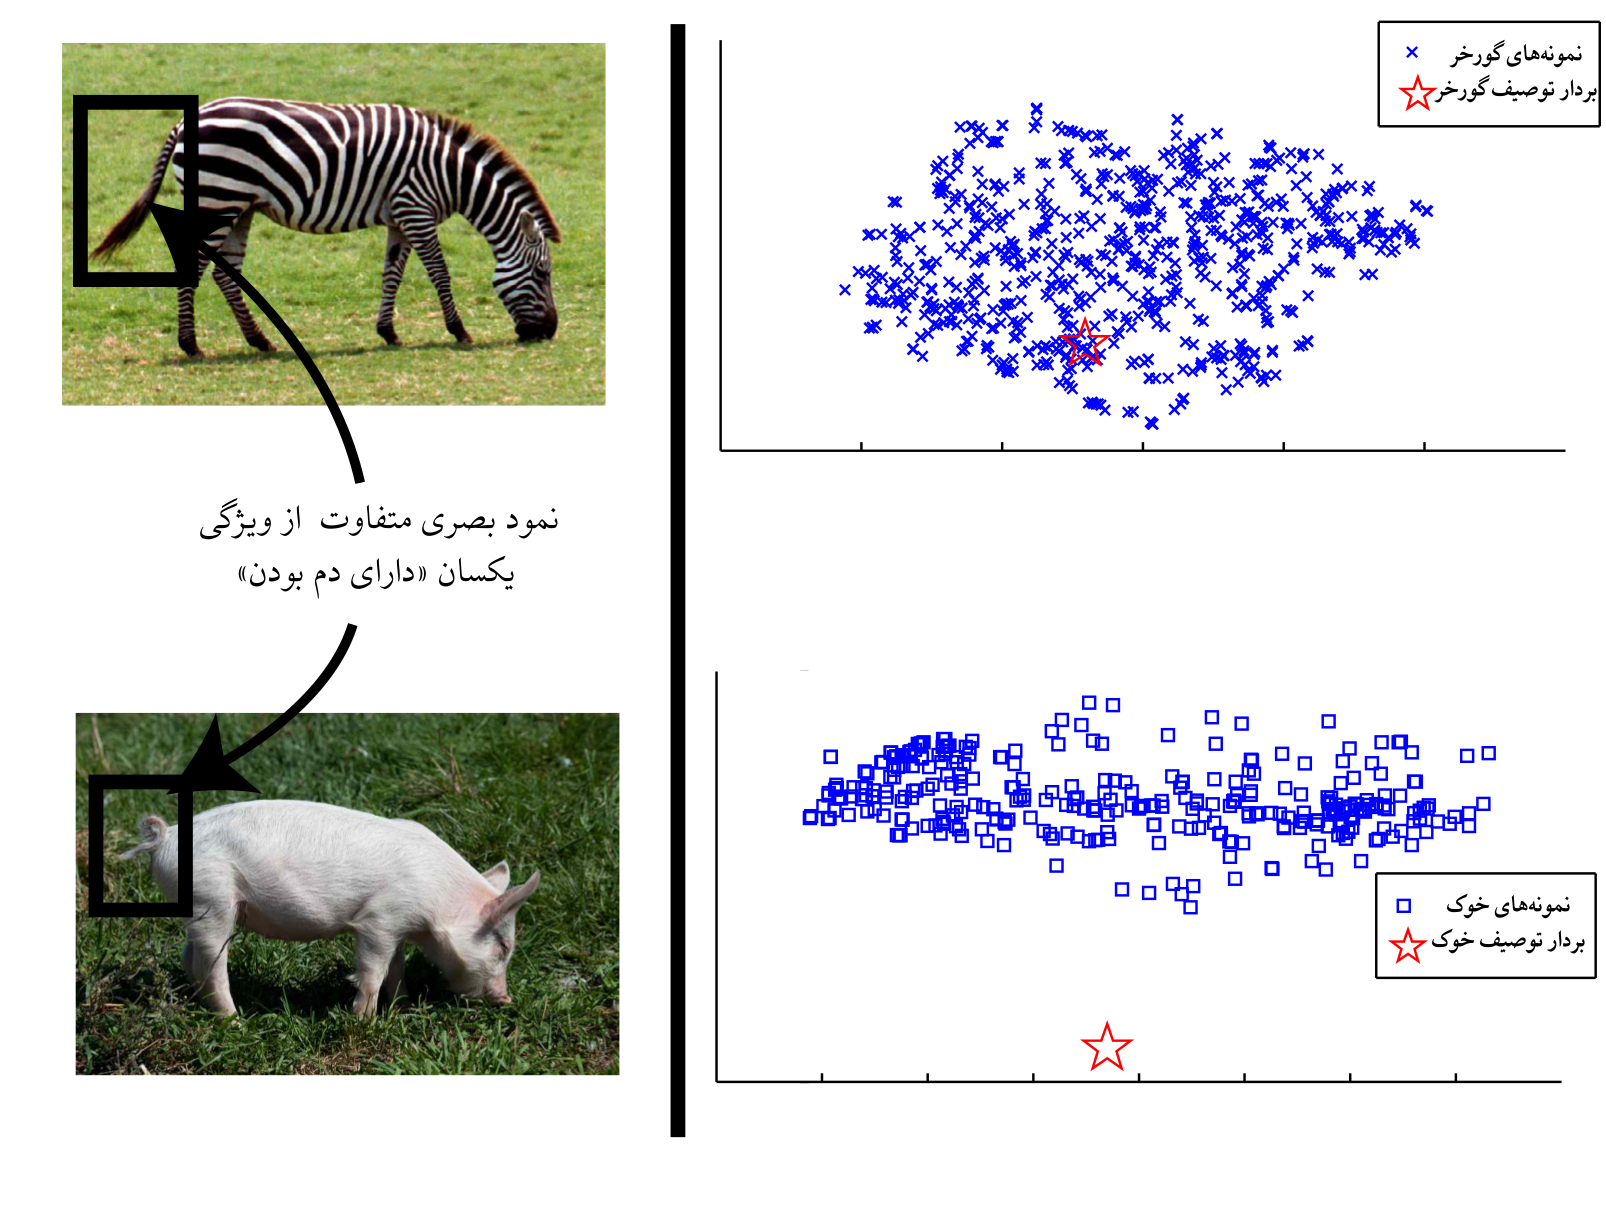
\includegraphics[width=0.7\linewidth]{images/domain_shift}
\caption[مشکل جابجایی دامنه]{
مشکل جابجایی دامنه بین دو دسته‌ی دیده شده (گورخر) و دیده نشده (خوک) نمایش داده شده است. ویژگی یکسان «دارای دم بودن» در این دو دسته دارای دو نمود بصری متفاوت است (سمت چپ) و نگاشت یادگرفته شده برای بردن این ویژگی به فضای مشترک برای دسته‌ی دیده نشده عمل‌کرد ضعیف‌تری نسبت به دسته‌ی دیده شده به نمایش می‌گذارد (سمت راست) 
\cite{Fu2014}.}
\label{fig:domain_shift}
\end{figure}
%-------------------------- Extendable
 در \cite{Fu2014} 
برای حل این مشکل دو تکنیک به کار گرفته شده است. ابتدا یافتن نمایش مشترک برای سه دامنه‌ی تصاویر، بردار ویژگی و بردار نام دسته‌ها به صورت توامان با استفاده از 
\lr{CCA}\LTRfootnote{Canonical Correlation Analysis}\cite{cca}
سپس برچسب‌گذاری داده‌های بدون برچسب در این فضای مشترک با استفاده از یک تکنیک انتشار برچسب\LTRfootnote{Label Propagation} بیزی. 

در \cite{li15max} 
مسئله به صورت یک دسته‌بندی روی دسته‌های دیده شده و خوشه‌بندی روی دسته‌های دیده‌نشده به صورت توام مدل شده است. در این روش یک دسته‌بند خطی روی تصاویر یادگرفته می‌شود که این دسته‌بند ترکیبی از پارامترهای مدل و توصیف‌هاست. به صورت دقیق‌تر چهارچوب یادگیری برابر خواهد بود با:
\begin{align}
\label{eq:max-margin}
\min_{Y, U, W, \boldsymbol{\xi}} \quad & \frac{\beta}{2} \normf{W}^2 + \frac{\beta}{2} \normf{U}^2 + \mathbf{1}^T \boldsymbol{\xi} \\
s.t. \quad & diag \big( ( Y - \mathbf{11}_k^T) \big) UWX^T) \geq (\mathbf{1} - Y\mathbf{1}_k) - \boldsymbol{\xi}, \, \forall k \in \mathcal{Y} \\
& Y \in \{0,1\}^{(N_s+N_u)\times(n_s + n_u)}, \quad BY = Y_s^T,  \label{eq:constraint_y1}\\
& Y\mathbf{1} = \mathbf{1}, \quad l \mathbf{1} \leq Y^T \mathbf{1} \leq h\mathbf{1} \label{eq:constraint_y2}
\end{align}
که در این صورت‌بندی فوق، $U$ را می‌توان توصیف‌های موجود برای هر دسته در نظر گرفت،
$Y$ برچسب‌ها را نشان می‌دهد و $B$ یک ماتریس انتخاب‌گر است که قسمتی از $Y$ را که مربوط به نمونه‌های آموزش است انتخاب می‌کند. $\beta$ و $l$ و $h$ فراپارامترهای مدل هستند که $\beta$ وزن جمله منظم‌سازی را تعیین می‌کند و $l$  و$h$ حداقل و حداکثر نمونه‌هایی که باید هر دسته دریافت کند را تعیین می‌کنند.
یک خاصیت جالب این صورت‌بندی این است که اگر دوگان مسئله بهینه‌سازی فوق را بنویسیم، $U$ تنها به شکل $UU^T$ ظاهر می‌شود، یعنی تنها اطلاعاتی که از دسته‌ها نیاز است میزان شباهتشان به یکدیگیر است که ممکن است از روی کواریانس توصیف‌ها محاسبه شود، اما در نبود توصیف به صورت مستقیم هم قابل بیان است.
در این چهارچوب اگر $U$ را ثابت در نظر بگیریم، $W$ یک دسته‌بندی $SVM$ روی دسته‌های دیده شده انجام می‌دهد و یک خوشه‌بندی روی دسته‌های دیده نشده. ضعف این چهارچوب در عدم استفاده از اطلاعات موجود در موقعیت مکانی داده‌های آزمون در خوشه‌بندی انجام شده روی آن‌هاست و هم‌چنین مسئله بهینه‌سازی تعریف شده برای داده‌های واقعی یک مسئله سخت است که به منابع زمانی و محاسباتی زیادی نیاز دارد. برای حل مشکل اول، نویسندگان این پژوهش نوع دیگری از چهارچوب فوق ارائه می‌کنند که با اضافه کردن یک جمله هموار سازی  اطلاعات نزدیکی مکانی نمونه‌ها را وارد می‌کند.
\begin{align}
\label{eq:semi-super}
\min_{Y, U, W} \quad & \sum_{i=1}^{N_s + N_u} \ell(X_{(i)}^T W, Y_iU) + \frac{\alpha}{2} \normf{W}^2 + \frac{\beta}{2} \normf{U - U_0}^2 
+ \frac{\rho}{2} tr(Y_u L Y_u^T) \\
s.t. \quad & \eqref{eq:constraint_y1}, \, \eqref{eq:constraint_y2} \nonumber
\end{align}
که در آن $\alpha$ و $\rho$ فراپامترهای جملات منظم‌سازی هستند و $U_0$ ماتریس توصیف دسته‌هاست.  $L$ ماتریس لاپلاسین یک ماتریس مشابهت میان نمونه‌هاست که در اینجا عکس فاصله اقلیدسی نمونه‌ها در نظر گرفته شده است. به عبارتی اگر $A$ ماتریس متقارنی باشد که عکس فاصله دوبدوی نمونه‌های آزمون را از یکدیگر نشان می‌دهد، خواهیم داشت 
$ L = diag(A\mathbf{1}) - A$.
صورت‌بندی معادله \eqref{eq:semi-super} با صورت بندی انجام شده در \eqref{eq:max-margin} چند تفاوت دارد. اضافه شدن جمله لاپلاسین برای استفاده بهتر از اطلاعات موجود در نمونه‌های آزمون یکی از آن‌هاست. علاوه بر این، در این روش یادگیری نمایش برای برچسب‌ها همواره صورت می‌گیرد. این در حالی‌ست که در صورت‌بندی قبلی $U$ عموما برابر با توصیف‌های موجود در صورت مسئله در نظر گرفته می‌شد. در اینجا $U_0$ چنین مقداری را اختیار می‌کند و $U$ اجازه دارد تغییر کند تا نمایش بهتری یاد گرفته شود. این دو روش، علاوه بر نیمه‌نظارتی بودن، تفاوت مهم دیگری با سایر روش‌های ارائه شده برای یادگیری بدون برد دارند: در این دو روش برچسب‌های داده‌های آزمون به طور مستقیم حدس زده می‌شوند و از روش‌هایی مثل نزدیک‌ترین همسایه یا انتشار برچسب به عنوان یک مرحله جداگانه برای تعیین برچسب داده‌ها استفاده نمی‌شود. ضعف این روش‌ها سنگین بودن مسئله بهینه‌سازی تعریف شده است که به همین علت امکان استفاده از نمایش ابعاد بالا برای تصاویر که از شبکه‌های عمیق به دست می‌آید، از بین می‌رود.

در 
\cite{Kodirov2015}
مسئله یادگیری بدون برد به صورت یک مسئله تطبیق دامنه\LTRfootnote{Domain Adaptation} مدل می‌کند. مسئله دسته‌بندی به صورت بدون برد ذاتا یک مسئله تطبیق دامنه نیست. در مسئله تطبیق دامنه، یک پیش‌بینی یکسان روی داده‌هایی از دو دامنه متفاوت انجام می‌شود؛ حال آن‌که در مسئله یادگیر بدون برد علاوه بر تفاوت دامنه در نمونه‌ها، پیش‌بینی‌ها نیز برد متفاوتی دارند و در دسته‌های یکسانی نمی‌گنجد. اگر مسئله یادگیری بدون برد را به شیوه یافتن توصیف از روی تصاویر، یا به عبارتی پیش‌بینی ویژگی نگاه کنیم، این مسئله یک مسئله استاندارد تطبیق دامنه بدون نظارت است؛ چرا که یک مجموعه ویژگی یکسان برای داده‌هایی از دو دامنه متفاوت پیش‌بینی می‌شوند. در این روش، از یادگیری لغت‌نامه\LTRfootnote{Dictionary Learning} برای پیش‌بینی ویژگی استفاده می‌شود و با معرفی دو جمله منظم‌سازی، مسئله تطبیق دامنه و مشکل جابجای دامنه در نظر گرفته می‌شوند. برای هر یک از دامنه‌ها یک لغت‌نامه یادگرفته می‌شود که این شامل نمایش هر یک از ویژگی‌ها در فضای تصاویر است. سپس هر تصویر با توجه به اینکه چه میزان از هر ویژگی در آن وجود دارد، به صورت ترکیب این پایه‌ها بیان می‌شود. برای دامنه دسته‌های دیده شده، با توجه به این که ویژگی‌ها از پیش دانسته شده است، مسئله در حقیقت یافتن یک نگاشت خطی است، نه یادگیری یک لغت‌نامه:
\begin{equation}
\label{eq:dic_source}
  D_s = \argmin_{D_s} \normf{X_s - D_s Z_s}^2 + \gamma \normf{D_s}^2, \quad s.t. \, \normtwo{D_{(i)}} \leq 1
\end{equation}
که $\gamma$ یک فراپامتر و $D_s$ نگاشت خطی مورد نظر یا به عبارتی پایه‌های لغت‌نامه است.
برای دامنه آزمون، ویژگی‌های تصاویر دانسته نیستند در نتیجه یک مسئله یادگیری لغت‌نامه داریم که باید ویژگی‌ها همراه با  پایه‌های لغت‌نامه $D_u$ یادگرفته شوند:
\begin{align}
\label{eq:dic_target}
\{ D_u, Z_u \} =& \min_{D_u, Z_u} \normf{X_u - D_u Z_u}^2 + \lambda_1 \normf{D_u - D_s}^2 \\
&+ \lambda_2 \sum_{i,j} w_{ij}\normtwo{Z_{u(i)} - S_{u(j)}} + \lambda_3 \norm{Z_u}_1 \nonumber \\
s.t. \quad  &\normtwo{D_{(i)}} \leq 1 \nonumber
\end{align}
که در آن $\lambda_1$ و $\lambda_2$ و $\lambda_3$ فرا پارامترهای مدل هستند. $w_{ij}$ امتیاز شباهت نمونه‌ی $X_u(i)$ به دسته‌ی $j$ از دسته‌های دیده نشده است که با روش IAP بدست آمده است. در تابع هزینه‌ی فوق، جمله‌ی اول و آخر، جملات معمول مربوط به یادگیری لغت‌نامه‌ی تنک هستند. جمله‌ی دوم برای تطبیق دامنه اضافه شده است و شبیه بودن پایه‌های لغت‌نامه را میان دو دامنه اعمال می‌کند. یعنی که نمایش بصری هر یک ویژگی‌های دو دامنه باید نزدیک به یکدیگر باشد. جمله سوم برای حل مشکل جابجای دامنه اضافه شده است. این جمله اجبار می‌کند که ویژگی‌های پیش‌بینی شده برای هر یک تصاویر به امضای دسته‌های آزمون مشابهت داشته باشد.
در این روش بعد از پیش‌بینی ویژگی‌های $Z_u$ برای تصاویر آزمون، از انتشار برچسب برای تعیین دسته‌ها استفاده می‌شود. مزیت این روش سادگی مسئله بهینه‌سازی تعریف شده نسبت به دیگر روش‌های نیمه‌نظارتی است. در انجام بهینه‌سازی تناوبی روی $D_u$ و $Z_u$، مسئله اول جواب بسته دارد و مسئله دوم یک رگرسیون لاسو\LTRfootnote{LASSO Regression} است که بسته‌های نرم‌افزاری زیادی برای آن وجود دارد. از طرفی متفاوت در نظر گرفتن $D_u$ و $D_s$ موجه به نظر نمی‌رسد. درست است که خواص بصری هر یک ویژگی‌ها برای هر دسته متفاوت است (مثل راه‌راه  بودن دسته‌های ببر و گورخر) ولی این تفاوت به دسته‌های دیده شده یا دیده‌نشده مرتبط نیست و بین دو دسته‌ی دیده شده یا دو دسته‌ی دیده نشده نیز وجود دارد.
%%%%%%%%%%%%%%%----------

%----------------------Semi supervised vocabulary informed learning
در \cite{Fu2016} روش نیمه‌نظارتی کلمه‌محور \lr{SS-Voc}\LTRfootnote{Semi-Supervised VOCabulary informed learning}  ارائه می‌شود که بجای استفاده از نمونه‌های بدون برچسب از توصیف‌هایی (که اینجا کلمه هستند) که نمونه‌ای از آن‌ها موجود نیست استفاده می‌کند. این روش با استفاده از چنین کلماتی سعی در رفع کردن چهار نقص در روش‌های دیگر را دارد. این چهار مورد عبارتند از: ۱) فرض جدا بودن دسته‌های آموزش و آزمون واقعی نیست و ممکن است در زمان آزمون نمونه‌هایی از دسته‌های دیده شده هم وود داشته باشد. ۲) مجموعه دسته‌های دیده نشده عموما کم‌تعداد است، در حالیکه در مسائل واقعی تعداد دسته‌های دیده نشده می‌تواند بسیار زیاد باشد. ۳) تعداد زیادی نمونه از دسته‌های دیده شده برای آموزش لازم است. ۴) دانش غنی موجود در رابطه معنایی کلمات (نام دسته‌ها) مورد استفاده قرار نمی‌گیرد. 
در این روش نگاشتی از تصاویر به فضای معنایی نمایش کلمات یادگرفته می‌شود که به صورت همزمان باید دارای سه خاصیت زیر باشد:
\begin{enumerate}
\item هر تصویر برچسب‌دار نزدیک به نمایش معنایی برچسب خود نگاشته شود.
\item 
نمایش هر تصویر در فضای کلمات به نمایش برچسب درست خود نزدیکتر باشد تا به سایر برچسب‌های موجود
\item 
نمایش هر تصویر در فضای کلمات به نمایش برچسب درست نزدیکتر باشد تا به سایر کلمات لغت‌نامه.
\end{enumerate}
معیار سومی که برشمرده شد تفاوت اصلی این روش با سایر روش‌هایی مثل
\cite{devise}
است که از تابع هزینه‌ی رتبه‌بند استفاده می‌کنند. در نظر گرفتن فاصله با کلماتی در مجموعه آموزش و آزمون وجود ندارند باعث می‌شود که این روش توانایی دسته‌بندی مجموعه باز\LTRfootnote{Open Set} 
 را هم داشته باشد، یعنی حالتی که دسته‌های آزمون از پیش تعیین شده نیستند.
  
 برای تامین خاصیت اول، از تابع هزینه‌ی بیشترین حاشیه استفاده می‌شود:
\begin{align}
\label{eq:svr}
&\left(|\xi|_{\epsilon}\right)_{j} =\mathrm{max}\left\{ 0,|W_{\star j}^{T}\mathbf{x}_{i}-\left(\mathbf{\mathbf{u}}_{z_{i}}\right)_{j}|-\epsilon\right\} \\
&\mathcal{L}_{\epsilon}\left(\mathbf{x}_{i},\mathbf{u}_{z_{i}}\right) =\mathbf{1}^{T}\mid\xi\mid_{\epsilon}^{2} 
\end{align}
که
 $|\xi|_{\epsilon}\in\mathbb{R}^{a}$
و 
$()_j$،
$j$مین 
عنصر بردار را نشان می‌دهد. این جمله  مشابه تابع هزینه رگرسیون بردار پشتیبان\LTRfootnote{Support Vector Regression} 
  است که با استفاده از جمله‌ی درجه ۲ هموار شده است.
  
  برای تامین موارد دوم و سوم برای نگاشت از جمله زیر استفاده می‌شود:
\begin{equation}
\mathcal{M}\left(\mathbf{x}_{i},\mathbf{u}_{y_{i}}\right)=\frac{1}{2}\sum_{v}\left[G+\frac{1}{2}D\left(\mathbf{x}_{i},\mathbf{u}_{y_{i}}\right)-\frac{1}{2}D\left(\mathbf{x}_{i},\mathbf{u}_{v}\right)\right]_{+}^{2}\label{eq:vocab_maximal_margin}
\end{equation}
که در آن $v$ نمایش یک کلمه در فضای معنایی است، $G$ متغیر مربوط به حاشیه است و $\left[\cdot\right]_{+}^{2}$ نشان‌دهنده‌ی تابع هزینه‌ی لولای هموار شده است\LTRfootnote{quadratically smoothed hinge loss}. برای این که بهینه‌سازی امکان‌پذیر باشد $v$ بجای کل کلمات لغت‌نامه تنها چند مقدار نزدیک به نمایش برچسب صحیح یعنی $c_{y_i}$ را اختیار می‌کند.
در نهایت  تابع هزینه‌ی پیشنهادی برای یادگرفتن نگاشتی با خواص فوق به این صورت تعریف شده است:
 \begin{equation}
 \label{eq:vocab_informed}
 W = \argmin_{W} \lambda \normf{W}^2 + \sum_{n=1}^{N_u} \alpha \mathcal{L}_{\epsilon} (\mathbf{x_i, c_{y_i}}) + (1-\alpha) \mathcal{M}(\mathbf{x_i, c_{y_i}})
 \end{equation}
 در نهایت در این روش با جایگزین کردن $c$ با $cV$ در تابع هزینه‌ی فوق، نگاشت $V$ روی توصیف‌ها نیز یاد گرفته می‌شود تا نمایش کلمات که با استفاده از مجموعه متن بدون برچسب بدست آمده، با توجه به برچسب‌های موجود در مسئله تنظیم دقیق شود.

\section{جمع‌بندی}\label{lr:conclusion}
در پایان این فصل به یک مقایسه کلی از روش‌های پیشین و مزایا و معایب آن‌ها می‌پردازیم که در جدول 
\ref{tab:PriorWorks}
آمده است.
\begin{center}
\begin{longtable}{|p{7cm}|p{2.5cm}|c|p{3cm}|} 
 \caption{ مقایسه مهم‌ترین روش‌های ارائه شده برای یادگیری از صفر}\label{tab:PriorWorks} \\
\hline
 \rl{مزایا و معایب} &
 \rl{نوع توصیف} &
\rl{سال ارائه}&
\rl{نام روش} \\
\endhead
\hline
\footnotesize \rl{+ارائه یک چارچوب نظام‌مند  } \newline \rl{+ امکان تعویض برخی قسمت‌ها مانند نوع دسته‌بند مورد استفاده} \newline 
 \rl{- مدل نکردن ارتباط میان ویژگی‌ها} \newline \rl{- در نظر نگرفتن خطای دسته‌بندی در آموزش}&
\footnotesize \rl{بردار ویژگی} &
\footnotesize 2009 &
\footnotesize \lr{DAP} \cite{lampert09} \\
\hline


\footnotesize \rl{+ عدم نیاز به توصیف صریح دسته‌ها } \newline \rl{+ ارائه یک کران نظری برای خطای دسته‌بندی} 
\newline \rl{+ امکان استفاده در یادگیری با نظارت یا بدون برد}
\newline  \rl{- عدم امکان استفاده از توصیف‌های دقیق‌تر و بسنده کردن به شباهت میان دسته‌ها} &
\footnotesize \rl{ شباهت دسته‌ها با هم} &
\footnotesize 2013 &
\footnotesize \rl{طراحی ویژگی برای دسته‌ها} \cite{Yu2013} \\
\hline

\footnotesize \rl{+ معرفی مسئله استفاده از توصیف متنی و جمع‌آوری مجموعه دادگان لازم} \newline \rl{+ استفاده از روش‌های تطبیق دامنه } \newline 
 \rl{+ امکان یادگیری دسته‌بند برای هر کلاس دیده نشده‌ی جدید} \newline \rl{- سادگی مدل تحلیل متن} \newline \rl{- محدود بودن به نگاشت‌های خطی} &
\footnotesize \rl{متن} &
\footnotesize 2013 &
\footnotesize \rl{دسته‌بند نوشتاری} \cite{mohamed13} \\
\hline

\footnotesize \rl{+ عدم نیاز به تهیه توصیف توسط انسان } \newline \rl{+ بهره‌گیری از پیش‌آموزش روی داده‌های فراوان} \newline \rl{- عدم دسته‌بندی دقیق برای دسته‌های نزدیک به هم} &
\footnotesize \rl{نام دسته‌ها}  &
\footnotesize 2013 &
\footnotesize \rl{DeViSE} \cite{devise} \\
\hline

\footnotesize \rl{+ معرفی مشکل جابجایی دامنه در یادگیری بدون برد و ارائه یک راه‌حل برای آن} \newline \rl{+ ارائه یک روش انتشار برچسب برای دسته‌بندی در مقابل نزدیک‌ترین همسایه } \newline 
 \rl{+ استفاده از چند توصیف به صورت همزمان} \newline \rl{- نیاز به داده‌های آزمون در زمان آموزش} &
\footnotesize \rl{بردار ویژگی و نام دسته‌ها} &
\footnotesize 2014 &
\footnotesize \rl{ نگاشت القایی چند منظری\LTRfootnote{Transductive Mult-View Embedding} } \cite{Fu2014} \\
\hline

\footnotesize \rl{+ در نظر گرفتن عدم قطعیت پیش‌بینی ویژگی در داده‌های آزمون} \newline \rl{+ تعمیم به مسئله یادگیری تک‌ضرب } \newline 
 \rl{- در نظر نگرفتن روابط بین ویژگی‌ها}  &
\footnotesize \rl{بردار ویژگی} &
\footnotesize 2014 &
\footnotesize \rl{ یادگیری بدون برد با ویژگی‌های غیرقطعی } \cite{jayaraman14} \\
\hline

\footnotesize \rl{+عدم نیاز به توصیف کلاس تهیه شده توسط انسان} \newline \rl{+ امکان انجام یادگیری از صفر چند برچسبی} \newline 
 \rl{- تنها امکان استفاده از اطلاع جانبی قابل دسته‌بندی}\newline \rl{- عدم امکان استفاده از ویژگی‌های غیر دودویی} &
\footnotesize\rl{ برچسب‌های دیگر}  &
\footnotesize 2014 &
\footnotesize \lr{COSTA} \cite{costa} \\
\hline

\footnotesize \rl{+ عدم نیاز به تهیه توصیف توسط انسان } \newline \rl{+ بهره‌گیری از پیش‌آموزش با داد‌های بدون برچسب فراوان} \newline 
\rl{+ عدم وجود فاز آموزش مخصوص به مسئله} 
\rl{+ امکان تشخیص برای هر دسته‌ی جدید} 
\rl{- عدم دسته‌بندی دقیق برای دسته‌های نزدیک به هم} &
\footnotesize \rl{نام دسته‌ها}  &
\footnotesize 2014 &
\footnotesize \rl{ConSE} \cite{convex} \\
\hline

\footnotesize \rl{+ درنظرگرفتن خطای دسته‌بند در آموزش} \newline \rl{+ دارای جواب بسته و پیاده‌سازی یک خطی} \newline 
 \rl{+ سرعت آموزش و آزمون بالا} \newline \rl{- محدود بودن رابطه به روابط خطی}&
\footnotesize \rl{بردار ویژگی} &
\footnotesize 2015 &
\footnotesize \lr{ESZSL} \cite{emb15} \\
\hline


\footnotesize \rl{+ امکان طبیعی استفاده از ویژگی‌ها با مقدار حقیقی} \newline \rl{+ ارائه یک روش عمومی برای بیان دسته‌های آزمون بر حسب دسته‌های آموزش } \newline \rl{- مسئله بهینه‌سازی نسبتا زمان‌بر} \newline \rl{- الزاما یکسان در نظر گرفتن توزیع داده‌های آموزش و آزمون}&
\footnotesize \rl{بردار ویژگی}  &
\footnotesize 2015 &
\footnotesize \lr{SSE} \cite{sse} \\
\hline

\footnotesize \rl{+ ارائه یک چارچوب کلی برای نگاشت به یک فضای مشترک} \newline
 \rl{+ ارائه یک روش برای نگاشت نام دسته‌ها} \newline 
 \rl{+ امکان طبیعی استفاده از ویژگی‌ها با مقدار حقیقی}
 \rl{- محدود بودن به نگاشت‌های دو خطی}&
\footnotesize \rl{ بردار ویژگی یا نام دسته‌ها}  &
\footnotesize 2015 &
\footnotesize \lr{SJE} \cite{Akata2015} \\
\hline



\footnotesize \rl{+ یادگیری نمایش برچسب‌ها طوری که متمایزکننده‌ی دسته‌ها شود} \newline \rl{+ دسته‌بندی روی تمام دسته‌های آموزش و آزمون } \newline \rl{+ امکان دسته‌بندی حتی بدون توصیف با یادگیری توصیف‌ها}  &%\rl{- }&
\footnotesize \rl{بردار ویژگی یا بدون توصیف}  &
\footnotesize 2015 &
\footnotesize \rl{یادگیری از صفر نیمه‌نظارتی با یادگیری نمایش برچسب‌ها} \cite{semi15} \\
\hline

\footnotesize \rl{+ پیش‌بینی مستقیم برچسب‌های نهایی} 
\newline \rl{+ صورت‌بندی نیمه‌نظارتی  } 
\newline \rl{- مسئله بهینه‌سازی سنگین}
\newline \rl{- عدم استفاده از ویژگی‌های مکانی تصاویر آزمون}
  &%\rl{- }&
\footnotesize \rl{بردار ویژگی}  &
\footnotesize 2015 &
\footnotesize \rl{یادگیری بدون برد با دسته‌بند حداکثر حاشیه} \cite{li15max} \\
\hline

\footnotesize \rl{+ صورت‌بندی مسئله به صورت یک مسئله تطبیق دامنه بدون نظارت} 
\newline \rl{+ استفاده از اطلاعات بدون‌نظارت موجود در داده‌های آزمون } 
\newline \rl{+ مسئله بهینه‌سازی سبک } 
\newline \rl{- نیاز به یک پیش‌بینی اولیه از یک روش دیگر به عنوان ورودی}
  &%\rl{- }&
\footnotesize \rl{بردار ویژگی یا نام دسته‌ها}  &
\footnotesize 2015 &
\footnotesize \rl{تطبیق دامنه بدون نظارت برای یادگیری بدون برد} \cite{Kodirov2015} \\
\hline


\footnotesize \rl{+ معرفی دسته‌بند کانولوشنال}
\rl{+ صورت‌بندی مسئله با شبکه‌های عصبی}
 \newline \rl{- استخراج ویژگی‌های نه چندان خوب از متن} \newline 
\rl{- تعداد پارامترهای زیاد مدل}
 &
\footnotesize \rl{متن}  &
\footnotesize 2015 &
\footnotesize \rl{پیش‌بینی دسته‌بند از متن توصیفی} \cite{ba2015} \\
\hline

\footnotesize \rl{+ امکان طبیعی استفاده از انواع ویژگی‌های پیوسته} \newline \rl{+ پارامترهای مستقل از تعداد دسته‌ها } \newline \rl{- استنتاج سنگین که به اجبار تخمین زده می‌شود} &
\footnotesize \rl{بردار ویژگی}  &
\footnotesize 2016 &
\footnotesize \rl{تشخیص هم‌دسته بودن توصیف و تصویر} \cite{agnostic} \\
\hline

\footnotesize \rl{+ در نظرنگرفتن فرض محدود کننده جدا بودن دسته‌های آزمون و آموزش} 
\newline \rl{+ استفاده از کلمات لغت‌نامه برای نیمه‌نظارتی کردن روش }
\newline \rl{+ کارکرد روش در مسائل یادگیری عادی، بدون برد و مجموعه باز }
\newline \rl{+ توانایی اجرا زمانی که دسته‌های آزمون بسیار زیاد هستند }
 \newline \rl{- عدم امکان استفاده از اطلاعات نظارتی قوی‌تر مثل بردار ویژگی‌ها} &
\footnotesize \rl{نام دسته‌ها}  &
\footnotesize 2016 &
\footnotesize \lr{SS-VOC} \cite{Fu2016} \\
\hline

\footnotesize \rl{+ جمع‌آوری مجموعه دادگان متنی بزرگ} 
\newline \rl{+ استفاده از شبکه‌های عصبی بازگردنده\LTRfootnote{Recurrent}  برای تحلیل متن }
\newline \rl{+ ارائه یک فورمول‌بندی جامع بر اساس شبکه‌های عصبی با قابلیت یادگیری توامان تمام قسمت‌ها }
 \newline \rl{- عدم ارائه راه‌کار برای انتخاب معماری مدل متنی} &
\footnotesize \rl{متن}  &
\footnotesize 2016 &
\footnotesize \rl{یادگیری عمیق بازنمایی توصیف‌های متنی} \cite{Reed2016} \\
\hline

\footnotesize \rl{+ الگوریتم یادگیری آسان } 
\newline \rl{+ تشخیص ابعاد مهم نمایش متنی و کلمات مهم برای هر دسته }
 \newline \rl{- استخراج ویژگی خطی مدل ضعیفی برای داده‌های متنی است} &
\footnotesize \rl{متن}  &
\footnotesize 2016 &
\footnotesize \rl{یادگیری بدون برد از متون آنلاین با حذف نویز} \cite{lessismore} \\
\hline

\footnotesize \rl{+ استفاده از سطح دقیق‌تری برای تناظر میان تصویر و توصیف} 
\newline \rl{+ امکان استفاده از توصیف‌های متنی که بدون نظارت بدست می‌آیند }
\newline \rl{+ امکان استفاده همزمان از توصیف‌های مختلف }
 \newline \rl{- نیاز به اطلاعات نظارتی بیشتر در تصاویر برای تعیین قسمت‌های مختلف} 
 \newline \rl{- مسئله بهینه‌سازی با محدودیت‌های زیاد و سنگین} &
\footnotesize \rl{توصیف‌های گوناگون}  &
\footnotesize 2016 &
\footnotesize \rl{یادگیری بدون برد با چند راهنما} \cite{multicue} \\
\hline


\footnotesize \rl{+ عدم محدودیت به نگاشت‌های خطی و در نظر گرفتن نگاشت‌های غیر خطی به صورت تکه‌تکه دوخطی } 
\newline \rl{+ امکان استفاده همزمان از توصیف‌های مختلف }
 &
\footnotesize \rl{توصیف‌های گوناگون}  &
\footnotesize 2016 &
\footnotesize \lr{LatEm} \cite{Xian2016} \\
\hline


\end{longtable}
\end{center}





































